% arara: pdflatex: {shell: yes, synctex: yes, options: "-file-line-error-style"}
% arara: bibtex if found('log', 'undefined references')
% arara: pdflatex: {shell: yes, synctex: yes, options: "-file-line-error-style"}
% arara: pdflatex: {shell: yes, synctex: yes, options: "-file-line-error-style"}

\documentclass{beamer}

\usetheme{default}

\usepackage{hyperref}
\usepackage{graphicx}
\usepackage{sidecap}

\title{Report on fire}
\author{Alber Sanchez}
\institute{TREES Lab - INPE}
\date{\today}



\begin{document}


\frame{\titlepage}

\begin{frame}{Overview}
    \tableofcontents
\end{frame}

\AtBeginSection[]{
    \begin{frame}{Outline}
        \tableofcontents[currentsection]
    \end{frame}
}



%%%%%%%%%%%%%%%%%%%%%%%%%%%%%%%%%%%%%%%%%%%%%%%%%%%%%%%%%%%%%%%%%%%%%%%%%%%%%%%
\section{Research questions}
%%%%%%%%%%%%%%%%%%%%%%%%%%%%%%%%%%%%%%%%%%%%%%%%%%%%%%%%%%%%%%%%%%%%%%%%%%%%%%%




\begin{frame}[t, allowframebreaks]
    \frametitle{Research questions}
    \begin{itemize}
        \item NEW QUESTIONS:
        \begin{itemize}
            \item How many DETER's Burned Area polygons fall inside PRODES?
            \item How many sucessive burns are needed for deforestation?
            \item How many DETER's areas don't have a heat spot?
            \item How much DETER's area doesn't have a heat spot?
            \item What is FireCCI's confidence required to make it match DETER?
            \item Are the burned areas counted more than once if they last long
                enoug?
        \end{itemize}
        \item DETER:
        \begin{itemize}
            \item Is DETER understimating burn area?
            \item How many yearly events happened before first mapping? How 
                many fires are needed for deforestation? Are burn scars 
                actually re-burns?
            \item How does DETER compare to INPE's \textit{Quemaidas}?
            \item How is deforestation by sucessive degradation shown in DETER?
            \item Can a burned area be on fire more than once?
            \item How do fire events relate to PRODES and TERRACLASS?
        \end{itemize}
        \item OTHER:
        \begin{itemize}
            \item How do we avoid counting each fire more than once? 
            \item How do we prepare fire data to feed a GHG emission model?
            \item How do fire maps compare? NOTE: Validate fire products. 
            \item Can we merge this data products to improve GHG emission 
                estimations?
            \item Is a burn scar actually a re-burn?
            \item Is fire re-occurrence really 60\%?
            \item Is it possible to link fires to burn scars?
            \item Can the heat focus be used to build a re-burn index?
            \item Is the fire product overestimating frequency?
            \item First fire is weak, probably they aren't mapped. What was the 
                time before the first detection? How many times did they burn 
                before first detection? Check Norton' paper 2011.
            \item How are the fire events characterized (shape, area, 
                detection interval)?
        \end{itemize}
    \end{itemize}
\end{frame}



%%%%%%%%%%%%%%%%%%%%%%%%%%%%%%%%%%%%%%%%%%%%%%%%%%%%%%%%%%%%%%%%%%%%%%%%%%%%%%%
\section{Projects}
%%%%%%%%%%%%%%%%%%%%%%%%%%%%%%%%%%%%%%%%%%%%%%%%%%%%%%%%%%%%%%%%%%%%%%%%%%%%%%%

\begin{frame}[t, allowframebreaks]
    \frametitle{PRODES}
    \begin{itemize}
        \item Unlike DETER, PRODES data doesn't explicitly label deforestation
            polygons as fire-scars.
    \end{itemize}
\end{frame}

\begin{frame}[t, allowframebreaks]
    \frametitle{DETER project~\cite{dealmeida2022}}
    \begin{itemize}
        \item Near Real Time alert system with low false-positive rate 
            (Amazon) coupled to IBAMA and law enforcement on the field. 
        \item Started in 2004 (PPCDAm).
        \item Areas larger than 3ha.
        \item Images:
        \begin{itemize}
            \item Based on optical remote sensing data.
            \item Until 2015, MODIS and CBERS-2B (250 m); min area 25ha.
            \item After 2015, CBERS-4, CBERS-4A, Amazonia-1; min area 3ha.
            \item Linear Mixture Model.
        \end{itemize}
        \item Method:
        \begin{itemize}
            \item Start with PRODES of last year, using water and 
                non-forest as exclusion mask.
            \item Photo-interpretation using soil fraction (end member?)
                and CBERS' RBG.
            \item Tone, color, shape, texture, and context.
            \item Polygons digitalized on-screen at 1:100,000 scale.
            \item Polygons are included daily. 
            \item Degradation polygons could be updated to deforestation.
            \item Data published weekly on Friday.
            \item DETER isn't meant for statistics.
        \end{itemize}
        \item Warning types: Deforestation and Degradation:
        \begin{itemize}
            \item Deforestation CR.
            \item Deforestation with vegetation
            \item Deforestation Mining.
            \item Degradation geometric selective cut.
            \item Degradation unordered selective cut.
            \item Degradation forest fire scar.
        \end{itemize}
    \end{itemize}
\end{frame}

\begin{frame}[t, allowframebreaks]
    \frametitle{DETER - Meeting with Marcos Adami}
    \begin{itemize}
        \item Why are fire scars collected by DETER? What for?
        \begin{itemize}
            \item Back in 2004 DETER used MODIS data. Then in 2008, polygons' 
                size fell, so they started using ISRO's ResourceSat. They 
                started using Spectral Mixture Model looking for selective 
                logging and fire because they thought it was interesting for
                IBAMA.
        \end{itemize}
        \item Could fire scars be duplicated? 
        \begin{itemize}
            \item Yes, but in different years, not in the same year.
        \end{itemize}
        \item Are the fire scars curated differently from other deforestation 
            polygons?
        \begin{itemize}
            \item No, all DETER's polygons are drawn using visual 
                interpretation on imagery and a Linear Mixture Model.
        \end{itemize}
        \item Are they underestimated? i.e. Fire was not detected by later 
            deforestation was.
        \begin{itemize}
            \item NA
        \end{itemize}
        \item What are the differences between DETER, DETER-B, and DETER 
            intenso?
        \begin{itemize}
            \item They are the same. However, DETER \textit{intenso} uses a ROI 
                and higher spatial resolution data, but it's not public.
        \end{itemize}
        \item What are DETER's recommended papers?
        \begin{itemize}
            \item DETER-R: An Operational Near-Real Time Tropical Forest 
                Disturbance Warning System Based on Sentinel-1 Time Series 
                Analysis.
        \end{itemize}
        \item Is it possible to get DETER data from 2015? 
        \begin{itemize}
            \item He is going to check the DB if the data is available and if
                there were changes in the mapping procedures before 2016.
        \end{itemize}
        \item DETER's Linear Mixture Model is made for the whole Amazonia, or
            for each State, or for each CBERS image?
        \begin{itemize}
            \item One LMM for each image.
        \end{itemize}
        \item Does DETER-R also identify burn scars? 
        \begin{itemize}
            \item No, DETER-R doesn't detect or use that label.
            %\item Marcos is going to check. As far as he understands, DETER-R 
                %is automatic.
        \end{itemize}
        \item Does DETER include DETER-R polygons?
        \begin{itemize}
            \item No, it does not.
        \end{itemize}
    \end{itemize}
\end{frame}



%%%%%%%%%%%%%%%%%%%%%%%%%%%%%%%%%%%%%%%%%%%%%%%%%%%%%%%%%%%%%%%%%%%%%%%%%%%%%%%
\section{Paper review}
%%%%%%%%%%%%%%%%%%%%%%%%%%%%%%%%%%%%%%%%%%%%%%%%%%%%%%%%%%%%%%%%%%%%%%%%%%%%%%%

\begin{frame}
    \frametitle{List of papers}
    \begin{itemize}
        \item \textit{Intercomparison of Burned Area Products and Its 
            Implication for Carbon Emission Estimations in the Amazon}
    \end{itemize}
\end{frame}



\begin{frame}[t, allowframebreaks]
    \frametitle{Long-Term Landsat-Based Monthly Burned Area Dataset for 
            the Brazilian Biomes Using Deep Learning~\cite{alencar2022}}
    \begin{itemize}
        \item MapBiomas Fire Collection 1.
        \item Use Machine Learning to map burned areas from 1985 to 2020 using
            Normalized Burn Ratio (NBR) on Landsat imagery.
    \end{itemize}
\end{frame}



\begin{frame}[t, allowframebreaks]
    \frametitle{Estimating Burned Area in Mato Grosso, Brazil, Using an 
    Object-Based Classification Method on a Systematic Sample of Medium 
    Resolution Satellite Images~\cite{shimabukuro2015}}
    \begin{itemize}
        \item This paper proposes a systematic sample in a degree grid (20 x20 
            Km) to assess burned area assessment.
        \item Estimate 2010s burned areas in Mato Grosso using JRC's 
            pan-tropical deforestation survey and cloud-free Landsat 5 imagery.
        \item Compare results to INPE's method (method 2) and to MCD64A1 
            (method 3).
        \item Method 1: Imagery preprocessing includes radiometric calibration, 
            dehazing, spectral normalization, cloud masking, multistage 
            segmentation of at least 5Ha.
        \item Method 2: Generate mixture model, segmentation of shade fraction,
            unsupervised classification, visual labeling (burned \& non-burned)
            edition of classification.
        \item Method 3: Use only MCD64A1 from before Landsat images' date. 
            Also, use MCD64A1 to estimate the proportion of total burned area. 
    \end{itemize}
    \begin{figure}
        \centering
        \includegraphics[width=0.7\textwidth]{./img/shimabukuro2015.png}
    \end{figure}
\end{frame}



\begin{frame}[t, allowframebreaks]
    \frametitle{Drought-driven wildfire impacts on structure and dynamics in a 
    wet Central Amazonian forest~\cite{pontes-lopes2021}}
    \begin{itemize}
        \item Field measures of trees at burned and unburned plots after a 
            wildfire, for 3 years, in the south of Manaus.
        \item Introduce questions about fire's behavior, structure, 
            demographics, and growth \& mortality drivers.
        \item What was the fire intensity and coverage?
        \item What was the magnitude of post-fire changes in stem density and 
            AGB and which growth forms and three sizes contributes to change?
        \item Which process drove the post-fire AGB dynamics?
        \item How did fire intensity and stem-level morphological attributes
            influence the post-fire growth of surveying trees and to what extent 
            did fire intensity and stem-level morphological attributes predict 
            tree and palm mortality after the fire, and how did the relative 
            importance of these predictors change over time?
    \end{itemize}
    \begin{figure}
        \centering
        \includegraphics[width=0.9\textwidth]{./img/pontes-lopes2022.png}
    \end{figure}
\end{frame}



\begin{frame}[t, allowframebreaks]
    \frametitle{A new global burned area product for climate assessment of fire 
    impacts: A new global burned area product~\cite{chuvieco2016}}
    \begin{itemize}
        \item This paper introduces Fire CCI.
        \item It uses the MERIS BA algorithm.
        \item Pixel (GeoTIFF) is a monthly, 300mts resolution, product 
            split by continent. It includes detection date, confidence, and 
            land cover (derived from Globcover2005).
        \item Burned Area (NetCDF-CF) is a 15-day, 0.5 degree resolution 
            product. It includes the total burned area, standard error, area 
            fraction, number of patches, and land cover.
        \item Cross-analysis with other BA products (2006-2008) used 
            spatio-temporal flooding algorithm and metrics perimeter to ratio, 
            ellipse elongation, azimutal angle, deviation from the North. The
            overall accuracy was 99.6\%.
        \item Fire CCI and Global Fire Emission Database BA produce comparable 
            results in simulations of fire emissions.
        \item Fire CCI Burned Area estimations have higher errors than MODIS BA
            products, but they are better balanced with less understimation 
            (close to 35\%).
        \item Available \href{https://climate.esa.int/de/projects/fire/}{here}.
    \end{itemize}
    \begin{figure}
        \centering
        \includegraphics[width=0.9\textwidth]{./img/firecci_comparison.png}
    \end{figure}
\end{frame}



\begin{frame}[t, allowframebreaks]
    \frametitle{Country-level fire perimeter datasets (2001 --- 2021)
    ~\cite{mahood2022}}
    \begin{itemize}
        \item Software \href{https://github.com/earthlab/firedpy}{FIREDpy}: 
            Downloads \& process MCD64A1 data using spatio-temporal flooding 
            (moving window)  to produce a fire perimeter SHP (daily or by 
            event). Source code available, it's also dokerized.
        \item Datasets: Created using FIREDpy, calibrated by region, and for 
            download by country.
        \item Download Brazil 
           \href{https://scholar.colorado.edu/concern/datasets/05741s90}{here}.
    \end{itemize}
    \begin{figure}
        \centering
        \includegraphics[width=0.7\textwidth]{./img/firedpy_comparison.png}
    \end{figure} 
\end{frame}



\begin{frame}[t, allowframebreaks]
    \frametitle{Tracking and classifying Amazon fire events in near real time
    ~\cite{andela2022}}
    \begin{itemize}
        \item There are 4 kinds of fires: Deforestation, leak fires, 
            agricultural management, and natural.
        \item Cluster fire detections into individual fires using Global Fire
            Atlas, VIRRS, Sentinel2, MODIS, GFED4.
        \item Multiday metrics and expert-guided classification.
        \item Method:
            \begin{itemize}
            \item This study combines active fire detections from VIIRS to map 
                the extent of individual fires using the Global Fire Atlas 
                    algorithm.
            \item It combines adjacent and sequential daily detections to 
                estimate fire behavior.
            \item Fires were classified into 4: Deforestation, Forest, Small 
                Clearing, and Savanna.
            \item It uses the fire season data of 2019.
            \item Fire data were combined to LULC to help fire classification.
            \item Fire classification was expert-guided because there was no 
                training data available.
            \item Classification validation using Monitoring of the Andean 
                Amazom project (MAAP) and Sentinel2 images.
            \item Estimation of GHG emissions by scaling data to match MCD64A1, 
                field work, and GFED.
        \end{itemize}
    \end{itemize}
\end{frame}



\begin{frame}[t, allowframebreaks]
    \frametitle{Mapping canopy damage from understory fires in Amazon forest
    using annual time series of Landsat and MODIS data}
    \begin{itemize}
        \item Burn Damage and Recover (BDR) algorithm.
        \item Southern Amazonia, Landsat (1997-2004) and MODIS (2000-2005).
    \end{itemize}
\end{frame}



\begin{frame}[t, allowframebreaks]
    \frametitle{Optimizing Near Real-Time Detection of Deforestation on 
    Tropical Rainforests Using Sentinel-1 Data~\cite{doblas2020}}
    NOTE: DETER-R doesn't distinguish deforestation from burn scars!
\end{frame}



\begin{frame}[t, allowframebreaks]
    \frametitle{DETER-R: An Operational Near-Real Time Tropical Forest 
    Disturbance Warning System Based on Sentinel-1 Time Series Analysis~\cite{doblas2022}}
    \begin{itemize}
        \item DETER-R doesn't separate deforestation for burn scars.
        % \item DETER-R doesn't mixture data with DETER. It's supposed to run in
        %     parallel with DETER.
        % \item DETER-R isn't publicly available.
        % \item DETER-R runs daily at 1AM BRT.
        % \item DETER-R needs two anomaluos SAR observations over a 2-month 
        %     time-series to confirm a warning.
        % \item DETER-R has a mean warning-issue delay of 24 days since first 
        %     perturbation.
        % \item DETER-R; less than 0.5\% of polygons are false positives.
        % \item Cloud cover is the main challenge to Near Real Time deforestation
        %     monitoring systems. However, radar isn't as sensible to clouds as
        %     optical imagery.
        % \item DETER-R uses Sentinel1 Radar images hosted and processed in 
        %     Google Earth Engine.
        % \item DETER-R is a forest disturbance detection method based on 
        %     time-series thresholding. The false-alert ration can be fixed by
        %     setting the number of standard deviations~\cite{doblas2020}.
        % \item This method make no assumptions about the non-forest 
        %     backscattering distribution.
        % \item DETER-R is an automated NRT forest disturbance detection 
        %     system based on Sentinel1 data hosted in Google Earth Engine. After
        %     automated analysis, forest disturbance pixel clusters are 
        %     vectorized and sent to environmental enforcement agencies.
        % \item GEE processing includes: Orbit correction, border and thermal
        %     noise removal, radiometric calibration, and terrain correction 
        % \item Forest extent comes from INPE, DLR, and IBGE.
        % \item Validation by visual inspection of optical images (Planet, 
        %     Sentinel2, Landsat).
        % \item Open source GEE 
        %     \href{https://mapbiomas.org/en/mapbiomas-fire-method}{scripts} 
        %     (Python).
        % \item DETER-R includes DETER data as a logistic model of distance to 
        %     deforestation (up to 10 km). Most new deforestation happens within 
        %     1km of old deforestation.
        % \item DETER-R uses time S1 time series to adjust a 3-year model 
        %     (learning collection) to compare to a 2-month data (detections 
        %     collection). Then it uses a threshold (logistic model) to detect
        %     any two consequtive inferior values as a confirmed detection.
        % \item Deforestation (polygons) smaller than 1ha are discarded. 
        % \item Polygons are labeled as low or high intensity depending on
        %     intensity of change.
        % \item Visual validation procedure. Compare DETER-R to DETER areas.
        % \item Alerts are sent to CENIMA IBAMA using FTP.
        % \item DETER-R was validated with field work in 2020.
    \end{itemize}
\end{frame}



\begin{frame}[t, allowframebreaks]
    \frametitle{Reference data accuracy impacts burned area product validation:
    the role of the expert analyst~\cite{franquesa2022}}
    \begin{itemize}
        \item Compare Burn Area obtained automatically to BA obtained by 
            interpreters.
        \item They compared FireCCI51 BA (Modis 250 m) to reference data 
            produced by interpreters on Sentinel2 images of the Amazon.
        \item Statistical analysis included:
            \begin{itemize}
                \item Difference Normalized Burned Area index (dNBR).
                \item Vegetation Continuous Field (VCF MOD44B v6).
                \item Canopy height from Global Forest Canopy Height (GFCH).
            \end{itemize}
        \item They found significant differences between FireCCI51 and 
            reference datasets.
        \item Disagreement between interpreters was more likely to occur in
            areas with low fire severity.
        \item Factors affecting accuracy of reference data: image quality,
            landscape composition, fire size and severity, image availability,
            subjectivity of the image interpreter.
        \item Low-severity burn areas generated greater uncertainty.
    \end{itemize}
    \begin{figure}
        \centering
        \includegraphics[width=1.0\textwidth]{./img/franquesa2022_roi.png}
    \end{figure}
\end{frame}

\begin{frame}
    \frametitle{A spatio-temporal active-fire clustering approach for global
    burned area mapping at 250 m from MODIS data}
    \begin{itemize}
        \item TODO.
        \item FireCCI51.
    \end{itemize}
\end{frame}


%%%%%%%%%%%%%%%%%%%%%%%%%%%%%%%%%%%%%%%%%%%%%%%%%%%%%%%%%%%%%%%%%%%%%%%%%%%%%%%
\section{Data}
%%%%%%%%%%%%%%%%%%%%%%%%%%%%%%%%%%%%%%%%%%%%%%%%%%%%%%%%%%%%%%%%%%%%%%%%%%%%%%%

\begin{frame}
    \frametitle{Mapbiomas Fire Collection 1}
    \begin{itemize}
        \item Brazil, Landsat (5, 7, \& 8), 1985-2020.
        \item Deep Neural Network clasification (Red, NIR, SWIR 1 \& 2, NDVI, 
            NBR, delta NBR) by biome, region (21) and 
            reference maps (MCD64A1 and INPE's \textit{Queimadas}).
        \item Sampling based on Annual classification mosaics (minimum NBR).
        \item Postprocessing included spatial filtering, fill small gaps (5,8 
            ha), remove small areas (1.4 ha).
        \item Method summary 
            \href{https://mapbiomas.org/en/mapbiomas-fire-method}{here}.
    \end{itemize}
\end{frame}

\begin{frame}
    \frametitle{MOD64A1}
\end{frame}

\begin{frame}
    \frametitle{Fire CCI}
\end{frame}

\begin{frame}
    \frametitle{Fabiano Morelli's data}
    Detect fire before and after the fire scar. 
    Link 
\end{frame}

\begin{frame}
    \frametitle{Global Fire Atlas}
\end{frame}

\begin{frame}
    \frametitle{Difference Normalized Burned Area index (dNBR)}
\end{frame}

\begin{frame}
    \frametitle{Vegetation Continuos Field (VCF - MOD44B v6)}
\end{frame}

\begin{frame}
    \frametitle{Canopy height from Global Forest Canopy Height (GFCH)}
\end{frame}

\begin{frame}
    \frametitle{VIIRS}
\end{frame}

\begin{frame}
    \frametitle{PRODES}
\end{frame}



\subsection{DETER}



% NOTE: Use fragile to avoid error caused by # in the URLs.
\begin{frame}[fragile]
    \frametitle{DETER data}
    \begin{itemize}
        \item Metadata \href{http://terrabrasilis.dpi.inpe.br/geonetwork/srv/por/catalog.search#/metadata/f2153c4a-915b-48a6-8658-963bdce7366c}{DETER shp}.
        \item Warnings of degradation and deforestation since August 2016.
        \item Deforestaion classes: Deforestation, deforestation with 
            vegetation, mining, 
        \item Degradation classes: Forest fire scar, degradation.
        \item Timber exploitation classes: Selective cutting type 1 (unplanned) 
            and 2 (planned).
        \item Date ranges from 2016-08-02 to 2022-07-29.
    \end{itemize}
\end{frame}



\begin{frame}
    \frametitle{DETER - Map of burn scars and warnings}
    \begin{figure}
        \centering
        \includegraphics[width=1.0\textwidth]{./img/deter_burn_scars.png}
    \end{figure}
\end{frame}



\begin{frame}
    \frametitle{DETER - Area by state and year}
    \begin{figure}
        \centering
        \includegraphics[width=1.0\textwidth]{./img/deter_warnings_area.png}
    \end{figure}
\end{frame}

\begin{frame}
    \frametitle{DETER - Warnings by state and year}
    \begin{figure}
        \centering
        \includegraphics[width=1.0\textwidth]{./img/deter_warnings_number.png}
    \end{figure}
\end{frame}

\begin{frame}
    \frametitle{DETER - Warnings by satellite, state, and year}
    \begin{figure}
        \centering
        \includegraphics[width=1.0\textwidth]{./img/deter_warnings_satellite.png}
    \end{figure}
\end{frame}



\begin{frame}
    \frametitle{BURN SCAR by area, state, type, and size}
    \begin{figure}
        \centering
        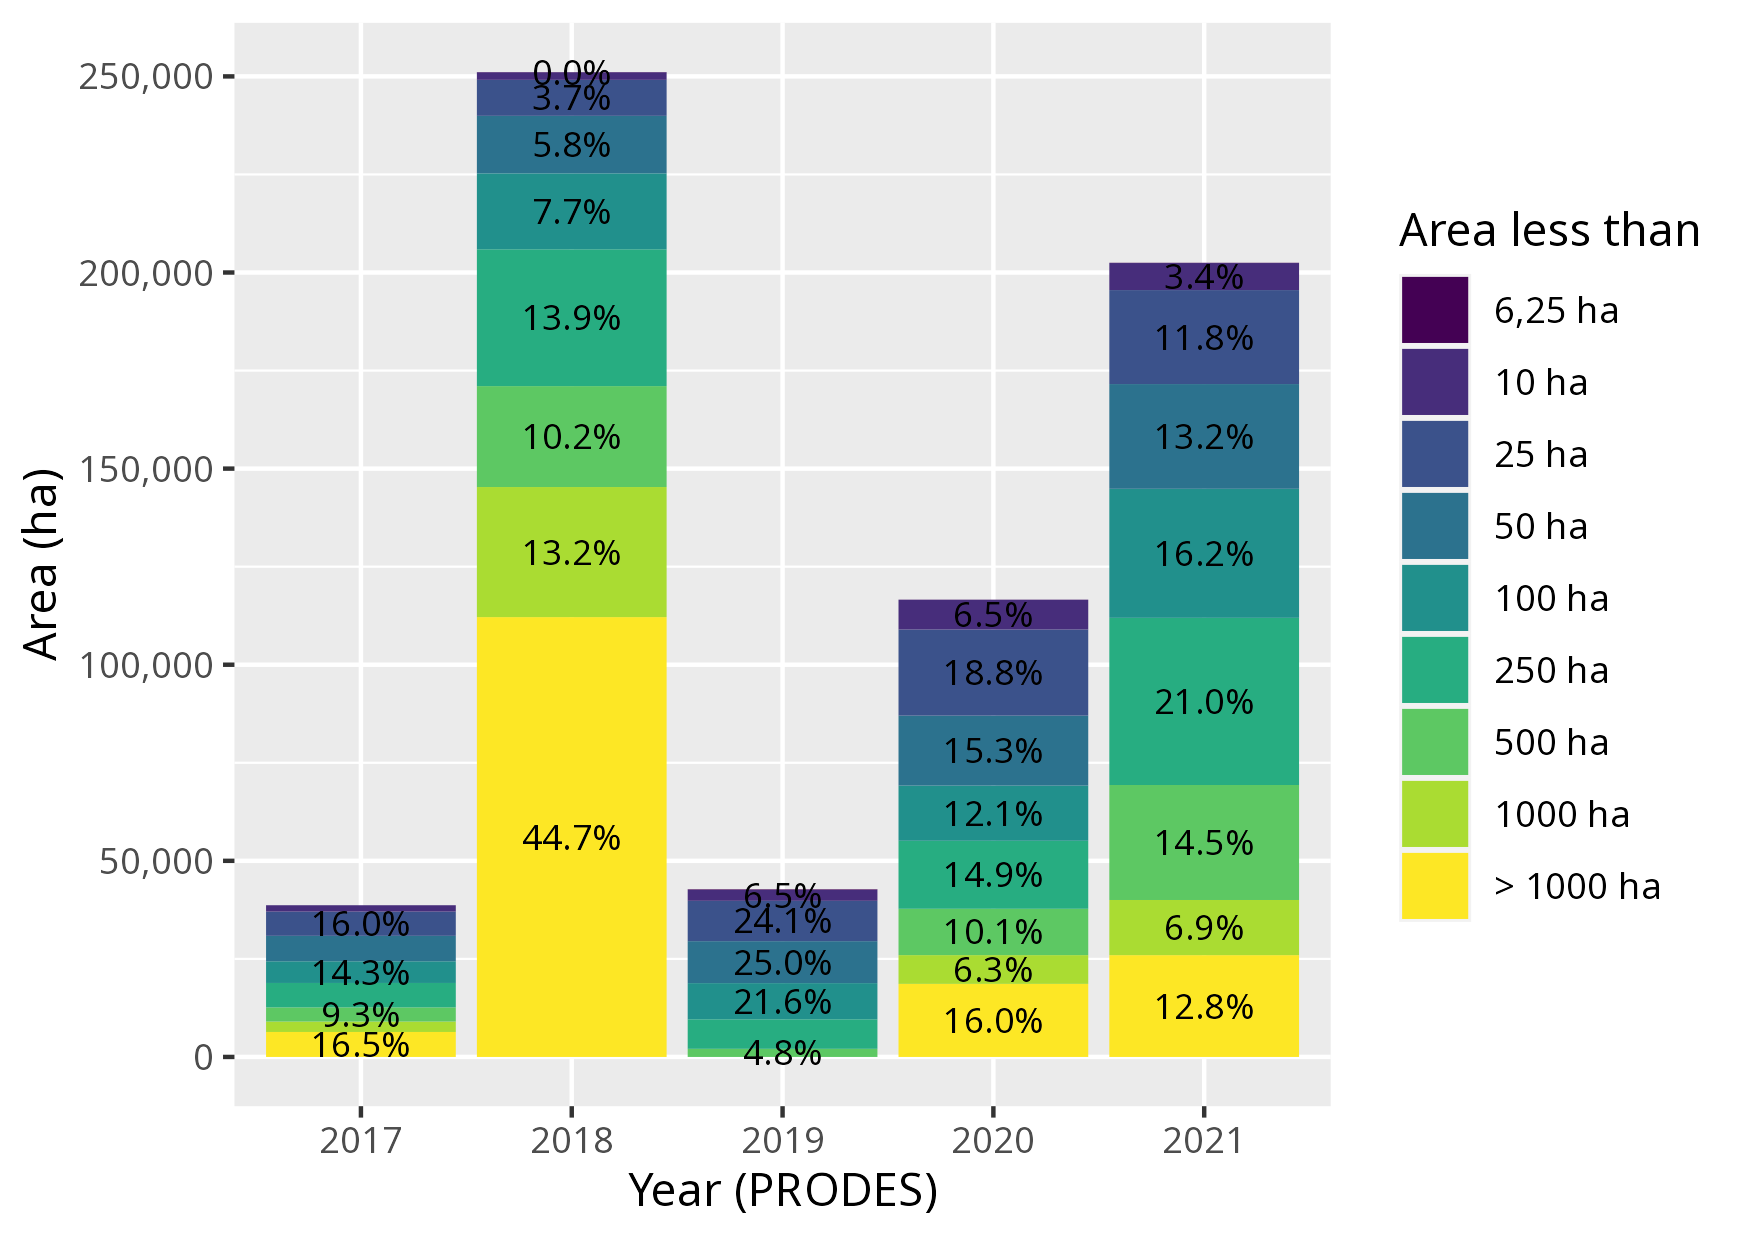
\includegraphics[width=1.0\textwidth]{./img/deter_warnings_area_size.png}
    \end{figure}
\end{frame}

\begin{frame}
    \frametitle{BURN SCAR events by state, type, and size}
    \begin{figure}
        \centering
        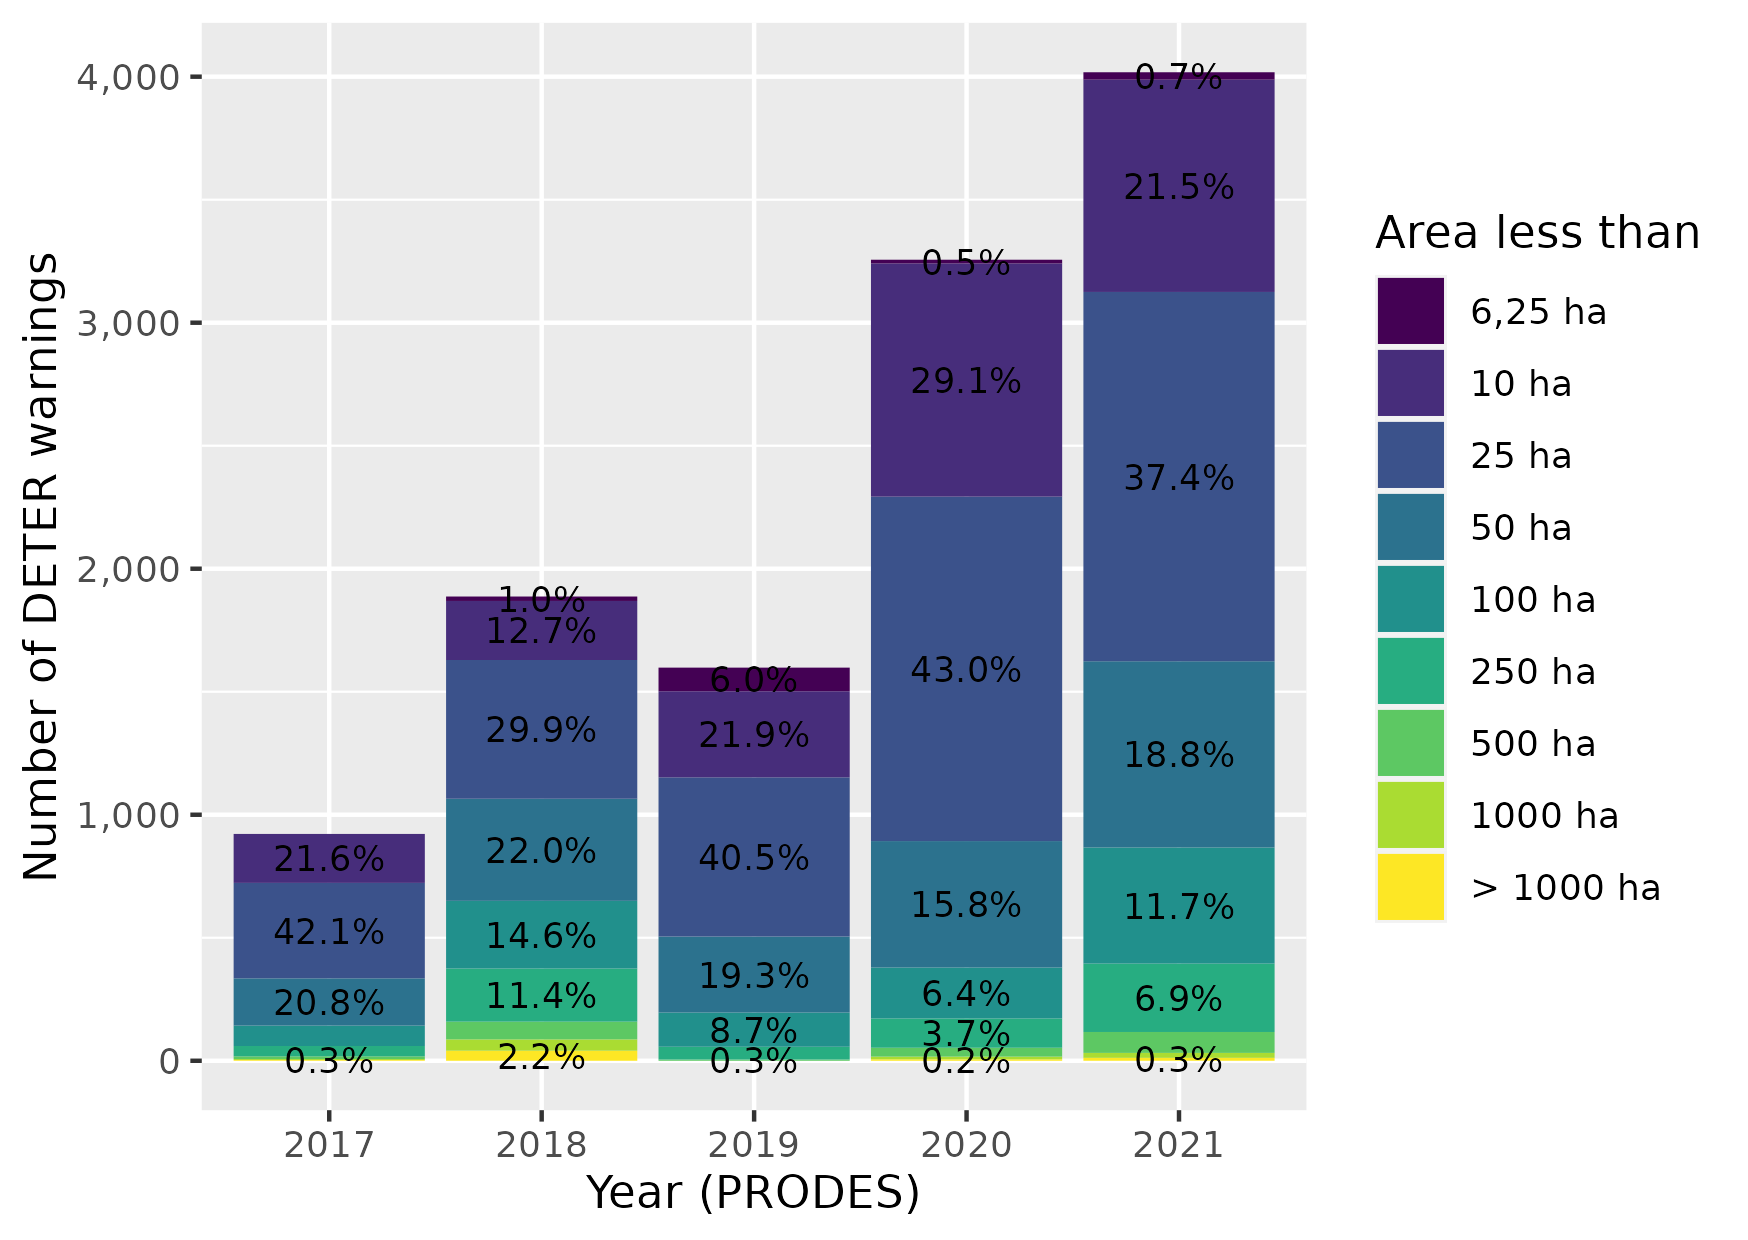
\includegraphics[width=1.0\textwidth]{./img/deter_warnings_size.png}
    \end{figure}
\end{frame}

\begin{frame}
    \frametitle{BURN SCAR area by state, and month}
    \begin{figure}
        \centering
        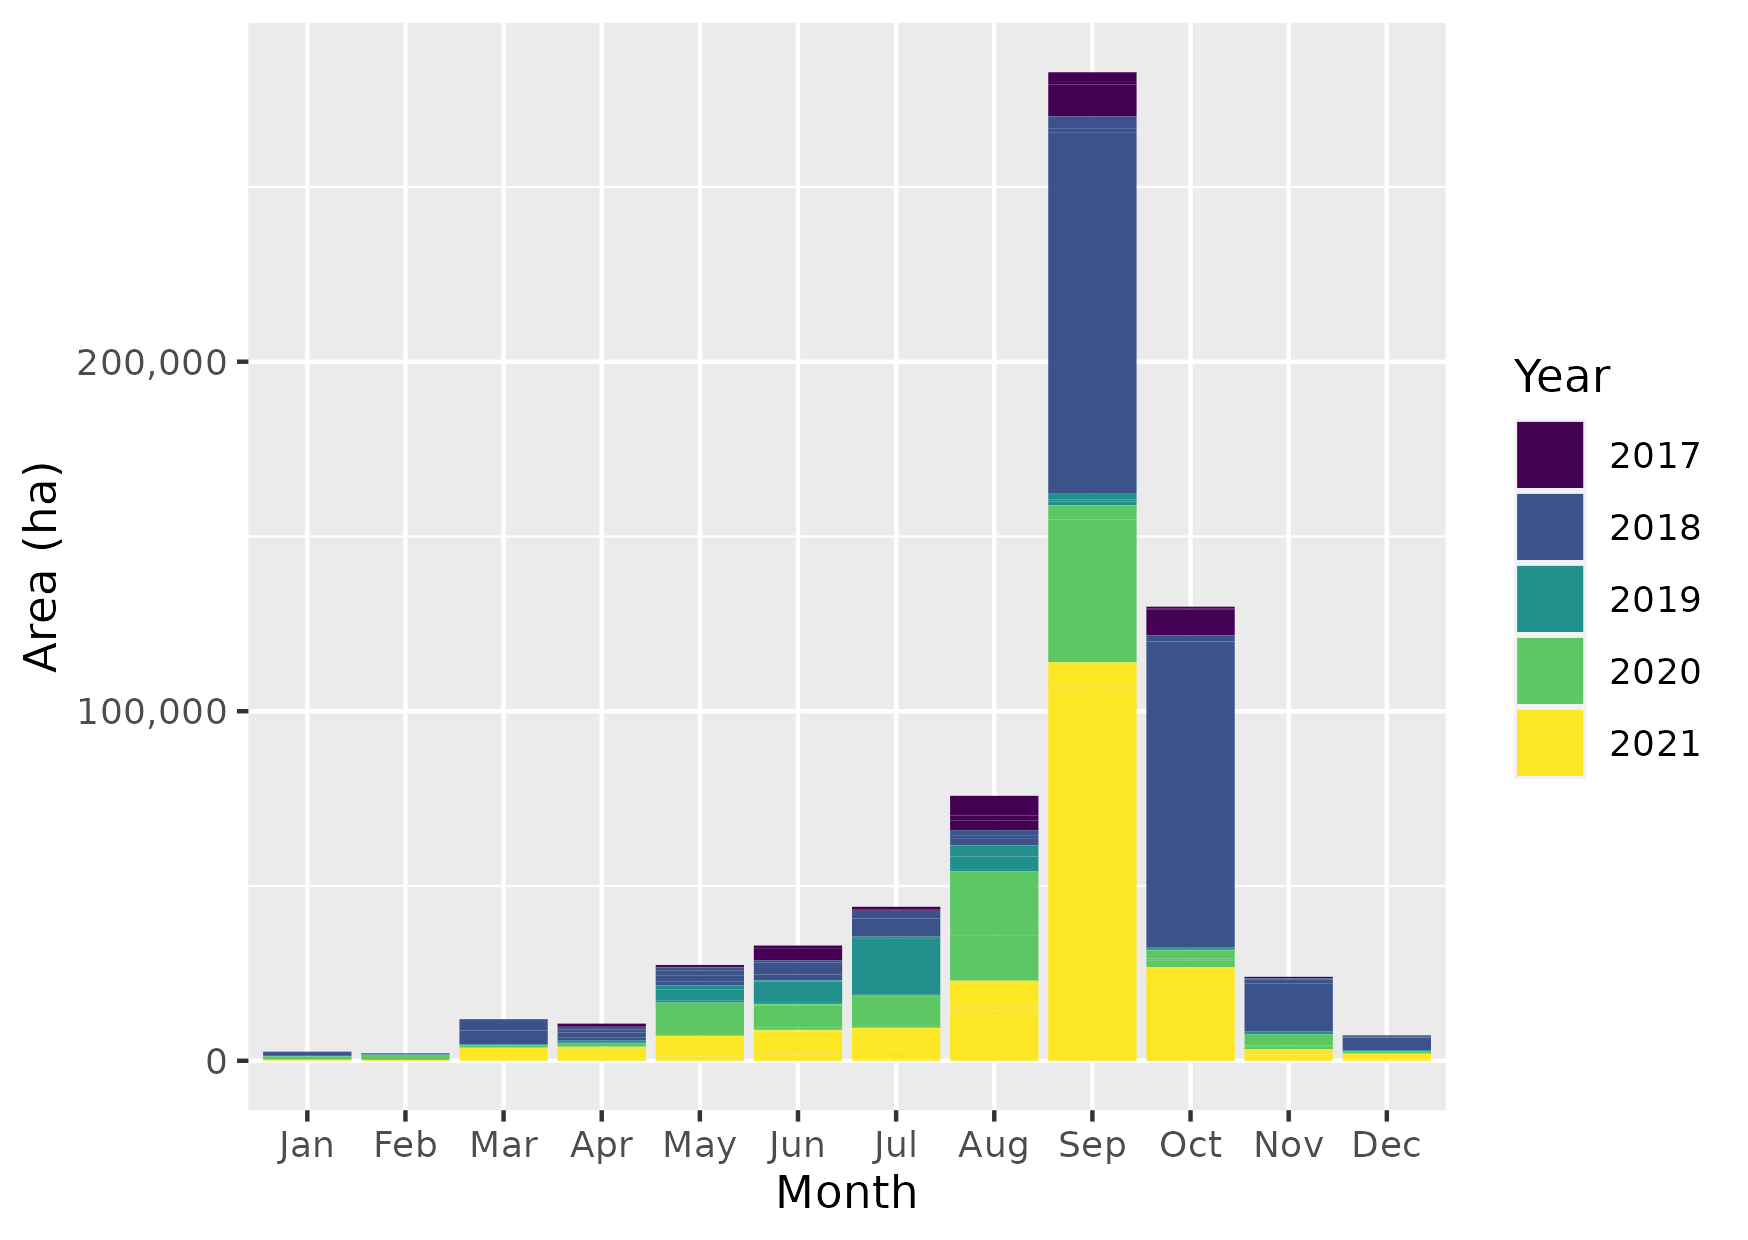
\includegraphics[width=1.0\textwidth]{./img/deter_warnings_size_month.png}
    \end{figure}
\end{frame}

\begin{frame}
    \frametitle{BURN SCAR events by state, and month}
    \begin{figure}
        \centering
        \includegraphics[width=1.0\textwidth]{./img/deter_events_size_month.png}
    \end{figure}
\end{frame}
  



%%%%%%%%%%%%%%%%%%%%%%%%%%%%%%%%%%%%%%%%%%%%%%%%%%%%%%%%%%%%%%%%%%%%%%%%%%%%%%%
\section{Software}
%%%%%%%%%%%%%%%%%%%%%%%%%%%%%%%%%%%%%%%%%%%%%%%%%%%%%%%%%%%%%%%%%%%%%%%%%%%%%%%

\begin{frame}
    \frametitle{R}
    \begin{itemize}
        \item R is ...
        \item Package R-GEE.
    \end{itemize}
\end{frame}

\begin{frame}
    \frametitle{Python}
    \begin{itemize}
        \item Python ...
        \item FIREDpy.
    \end{itemize}
\end{frame}

\begin{frame}
    \frametitle{JavaScript}
    \begin{itemize}
        \item JS is ...
        \item Google Earth Engine.
    \end{itemize}
\end{frame}



%%%%%%%%%%%%%%%%%%%%%%%%%%%%%%%%%%%%%%%%%%%%%%%%%%%%%%%%%%%%%%%%%%%%%%%%%%%%%%%
\section{Computing platforms}
%%%%%%%%%%%%%%%%%%%%%%%%%%%%%%%%%%%%%%%%%%%%%%%%%%%%%%%%%%%%%%%%%%%%%%%%%%%%%%%

\begin{frame}[t, allowframebreaks]
    \frametitle{Google Earth Engine EE101-B}
    \begin{itemize}
        \item 9 PB of public data (imagery, geophysical, weather forecast, 
            climate models) (2017).
        \item API: JavaScript and Python.
        \item Data Models: Feature,  Images, Collections.
        \item Feature: line, point, polygon, list of properties.
        \item Images: Stack of bands (mask, projection, resolution), a list of 
            properties (date, bbox).
            \item Collection: Bag of elements (table of features, directory of
            images).
        \item Map: Apply a function for each element of a collection (for each).
        \item Reduce: Apply a function to everything in a collection 
            (aggregation). We can reduce neighborhood, regions, feature 
            collections, to vectors.
        \item Band math.
        \item Computation: On the fly process, tile by tile. Scatter and 
            gather.
        \item Links:\href{https://youtu.be/m1ejxSi3l8s}{video}, 
            \href{goo.gl/ZUqPXz}{slides},
            \href{goo.gl/01kki0}{code}.
    \end{itemize}
\end{frame}



\begin{frame}[t, allowframebreaks]
    \frametitle{sepal.io}
    \begin{itemize}
        \item A powerful, open-source platform for forest and land monitoring.
        \item FAO's platform.
        \item Create and analyze data for any place on Earth.
        \item Generate and improve land use maps, analyze time series, run
            change detection, perform accuracy and area assessments.
    \end{itemize}
\end{frame}



%%%%%%%%%%%%%%%%%%%%%%%%%%%%%%%%%%%%%%%%%%%%%%%%%%%%%%%%%%%%%%%%%%%%%%%%%%%%%%%
\section{Challenges}
%%%%%%%%%%%%%%%%%%%%%%%%%%%%%%%%%%%%%%%%%%%%%%%%%%%%%%%%%%%%%%%%%%%%%%%%%%%%%%%

\begin{frame}[t, allowframebreaks]
    \frametitle{Big data}
    \begin{itemize}
        \item Big data.
    \end{itemize}
\end{frame}



\begin{frame}[t, allowframebreaks]
    \frametitle{Heterogeneous platforms}
    \begin{itemize}
        \item JavaScript, Python, R.
    \end{itemize}
\end{frame}



%%%%%%%%%%%%%%%%%%%%%%%%%%%%%%%%%%%%%%%%%%%%%%%%%%%%%%%%%%%%%%%%%%%%%%%%%%%%%%%
\section{Vocabulary}
%%%%%%%%%%%%%%%%%%%%%%%%%%%%%%%%%%%%%%%%%%%%%%%%%%%%%%%%%%%%%%%%%%%%%%%%%%%%%%%

\begin{frame}[t, allowframebreaks]
    \frametitle{Fire vocabulary}
    \begin{itemize}
        \item Deforestation: Land conversion by suppression of areas of 
            primary vegetation by antropogenic actions (PRODES
            ~\cite{dealmeida2022}). 
        \item Clear cut (corte raso): Complete remotion of forest cover in a 
            short time interval.
        \item Fire event.
        \item Fire spot.
        \item Burned area.
        \item Burned area signal persistence over time.
        \item Detection time.
        \item Occurrence time.
        \item Deforestation by successive degradation. It is slower than 
            deforestation, taking many years~\cite{dealmeida2022}.
    \end{itemize}
\end{frame}



%%%%%%%%%%%%%%%%%%%%%%%%%%%%%%%%%%%%%%%%%%%%%%%%%%%%%%%%%%%%%%%%%%%%%%%%%%%%%%%
\section{Code}
%%%%%%%%%%%%%%%%%%%%%%%%%%%%%%%%%%%%%%%%%%%%%%%%%%%%%%%%%%%%%%%%%%%%%%%%%%%%%%%

\begin{frame}
    \frametitle{Scripts for downloading data}
    \begin{itemize}
        \item Fire CCI
        \item MCD64A1
        \item Available at \url{https://github.com/albhasan/treesburnareas}
    \end{itemize}
\end{frame}

\begin{frame}
    \frametitle{Downloaded data}
    \begin{itemize}
        \item Fire CCI version 5.1 from 2001 to 2020 (258 tar.gz files)
        \item MCD64A1 collection 6.1 from 2000.11.01 to 2022.02.01 
            \begin{itemize}
                \item h10v09 256 files
                \item h11v08 218 files 
                \item h11v09  24 files
            \end{itemize}
        \item Mapbiomas fire (Google Earth Engine)
            \begin{itemize}
                \item Too slow when downloading by biome Amazonia (up to 12 
                    hours!)
                \item It seems the build the product each time is accessed.
                \item Is there any data storage? 
            \end{itemize}
    \end{itemize}
\end{frame}


%%%%%%%%%%%%%%%%%%%%%%%%%%%%%%%%%%%%%%%%%%%%%%%%%%%%%%%%%%%%%%%%%%%%%%%%%%%%%%%
\section{Partial results}
%%%%%%%%%%%%%%%%%%%%%%%%%%%%%%%%%%%%%%%%%%%%%%%%%%%%%%%%%%%%%%%%%%%%%%%%%%%%%%%

\begin{frame}
    \frametitle{Subareas}
    \begin{itemize}
        \item DETER warnings are available for download as a shapefile.
        \item Warnings are represented as polygons with a date.
        \item Some of these polygons partially overlap across time.
        \item The common area of overlapped polygons are called \emph{subarea}. 
    \end{itemize}
\end{frame}

%%%%

\begin{frame}
    \frametitle{DETER warnings by area, type, year, and state}
    \begin{itemize}
        \item The following figure shows the area of the warnings issued by 
            DETER from 2017 to 2021.
        \item Since some of these areas partially overlap, their total is
            larger than the actual monitored area.
        \item Burn scars are the predominant warnings in PA, MT, MA, RR, \& TO.
    \end{itemize}
\end{frame}

\begin{frame}
    \frametitle{DETER warnings by area, type, year, and state}
    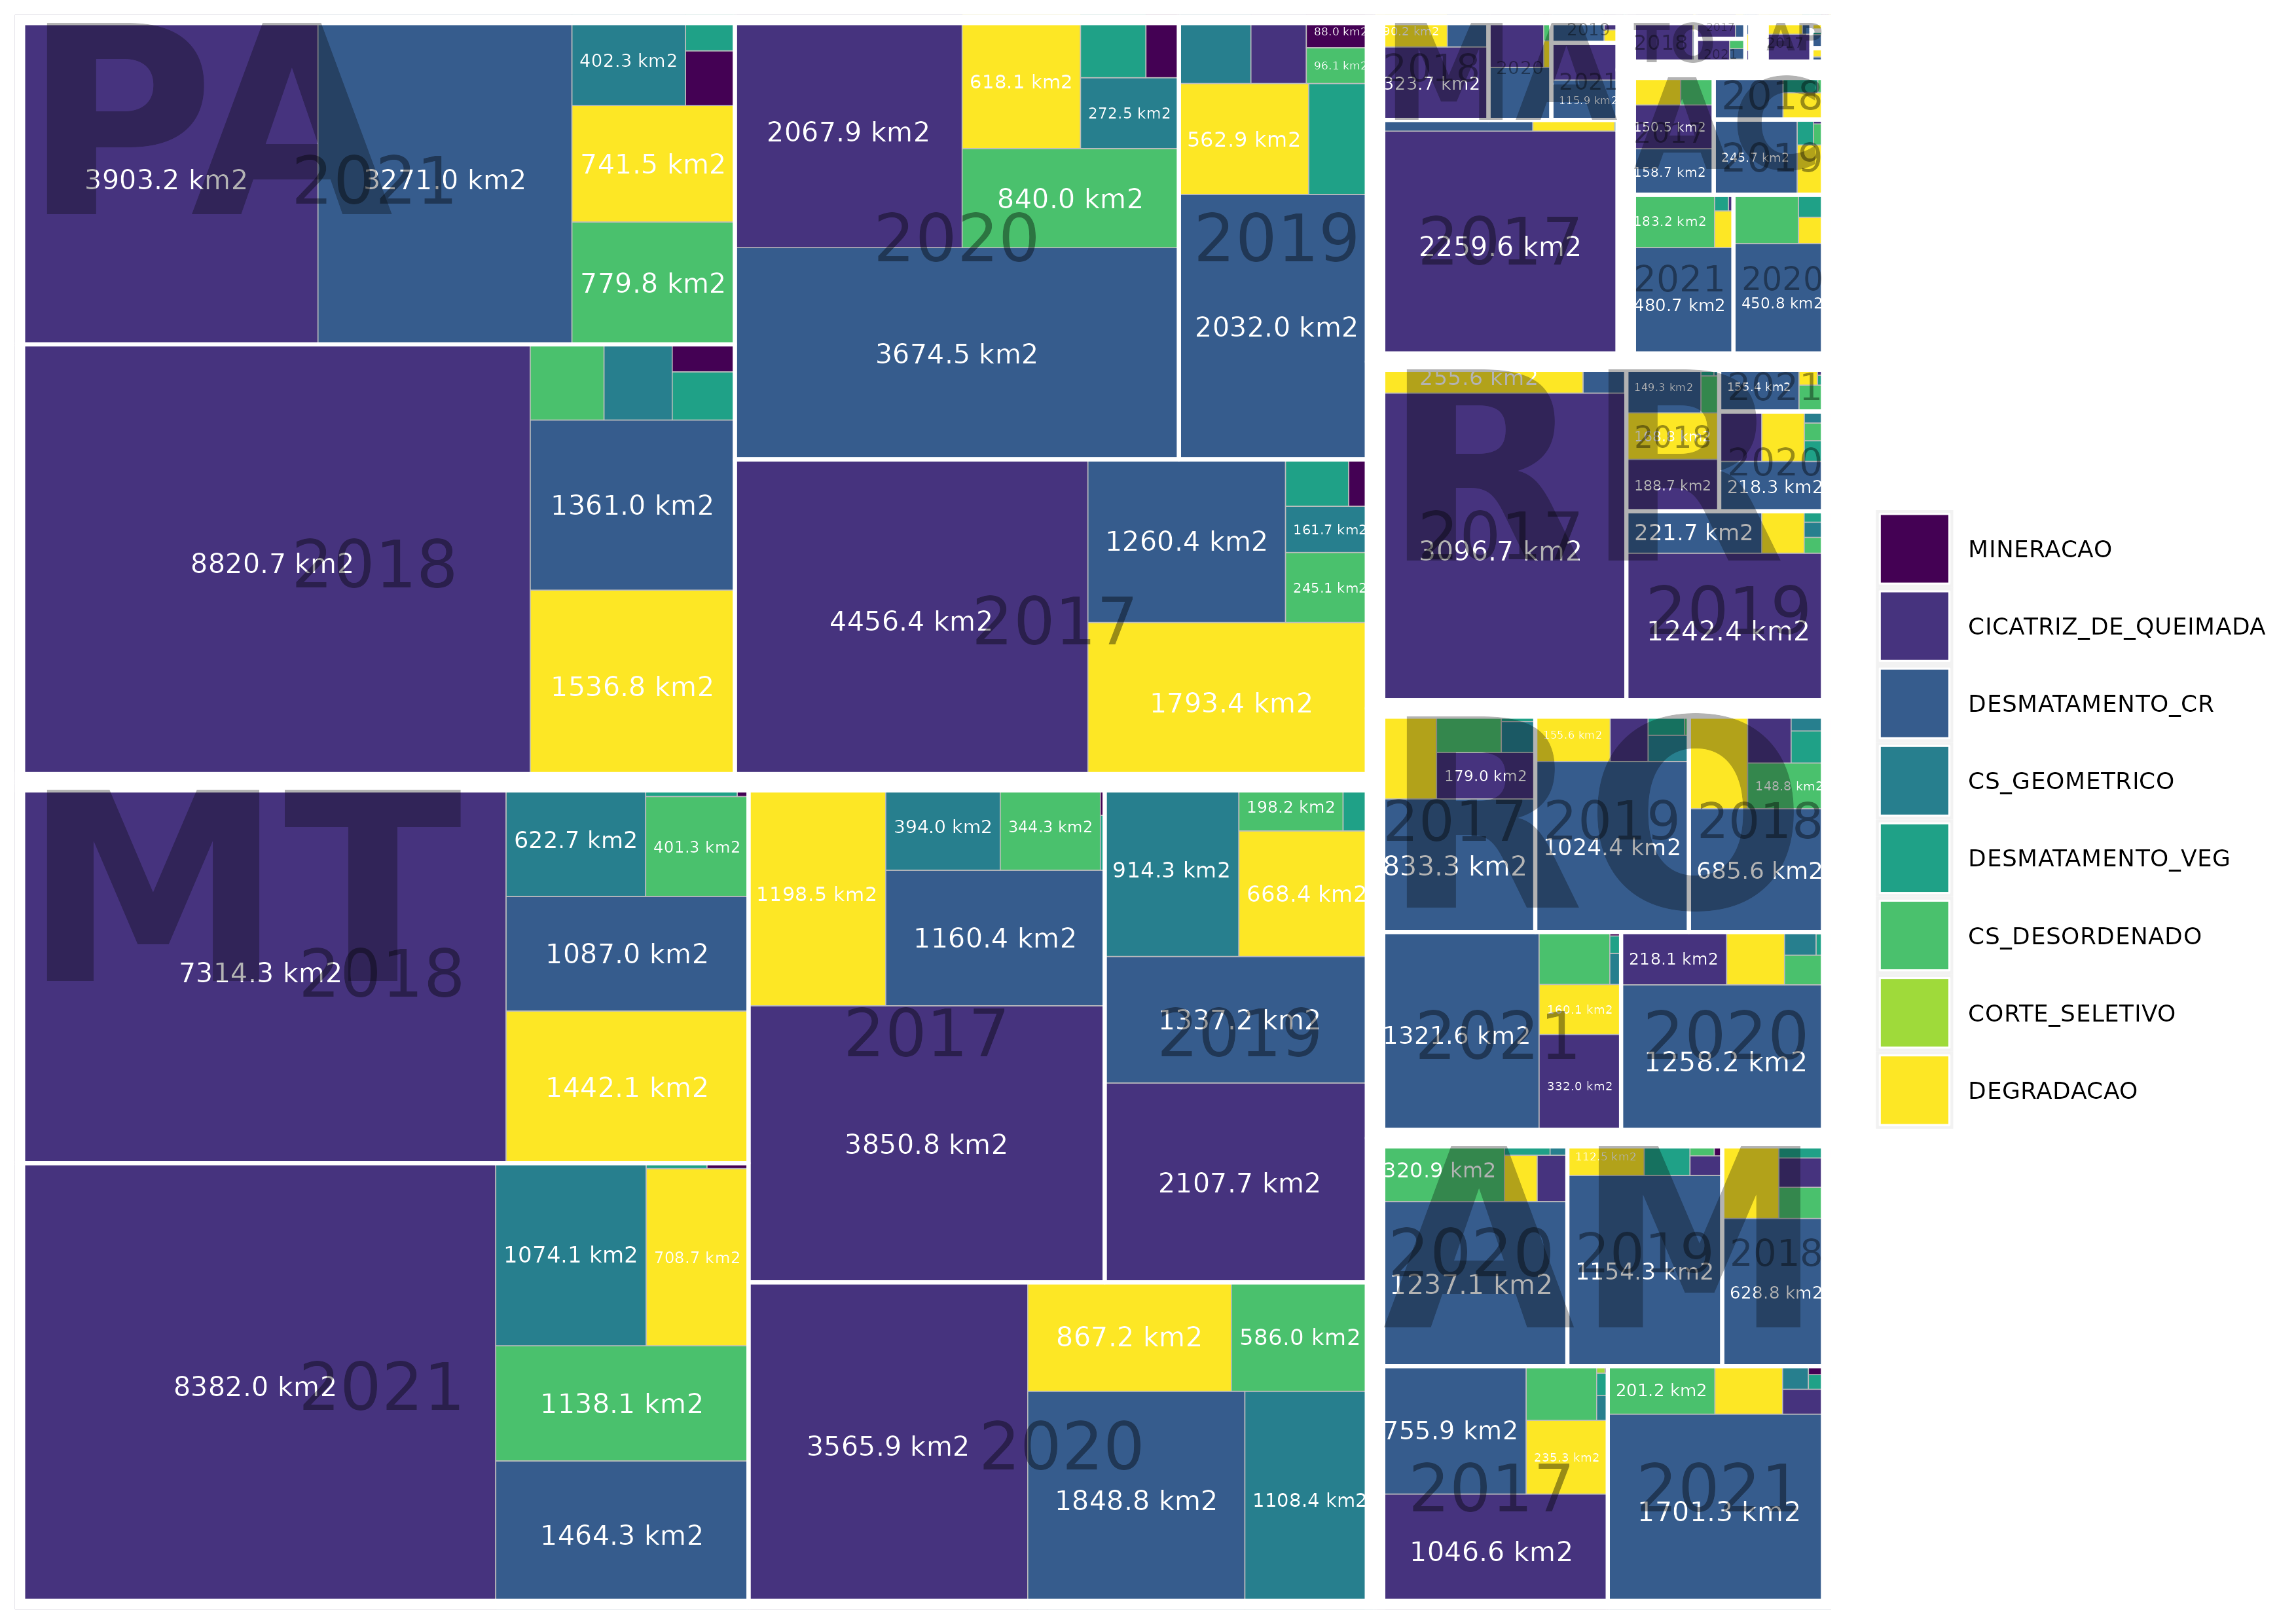
\includegraphics[width=1.0\textwidth]{./img_results/plot_deter_area_by_state_pyear_type.png}
\end{frame}

%%%%

\begin{frame}
    \frametitle{DETER warnings by subarea}
    \begin{itemize}
        \item The following 2 figures show DETER subarea (classified by size) 
            by number of warnings.
        \item The areas included in this figure do not overlap.
        \item The area intervals are almost logarithmic.
    \end{itemize}
\end{frame}

\begin{frame}
    \frametitle{DETER warnings by subarea}
    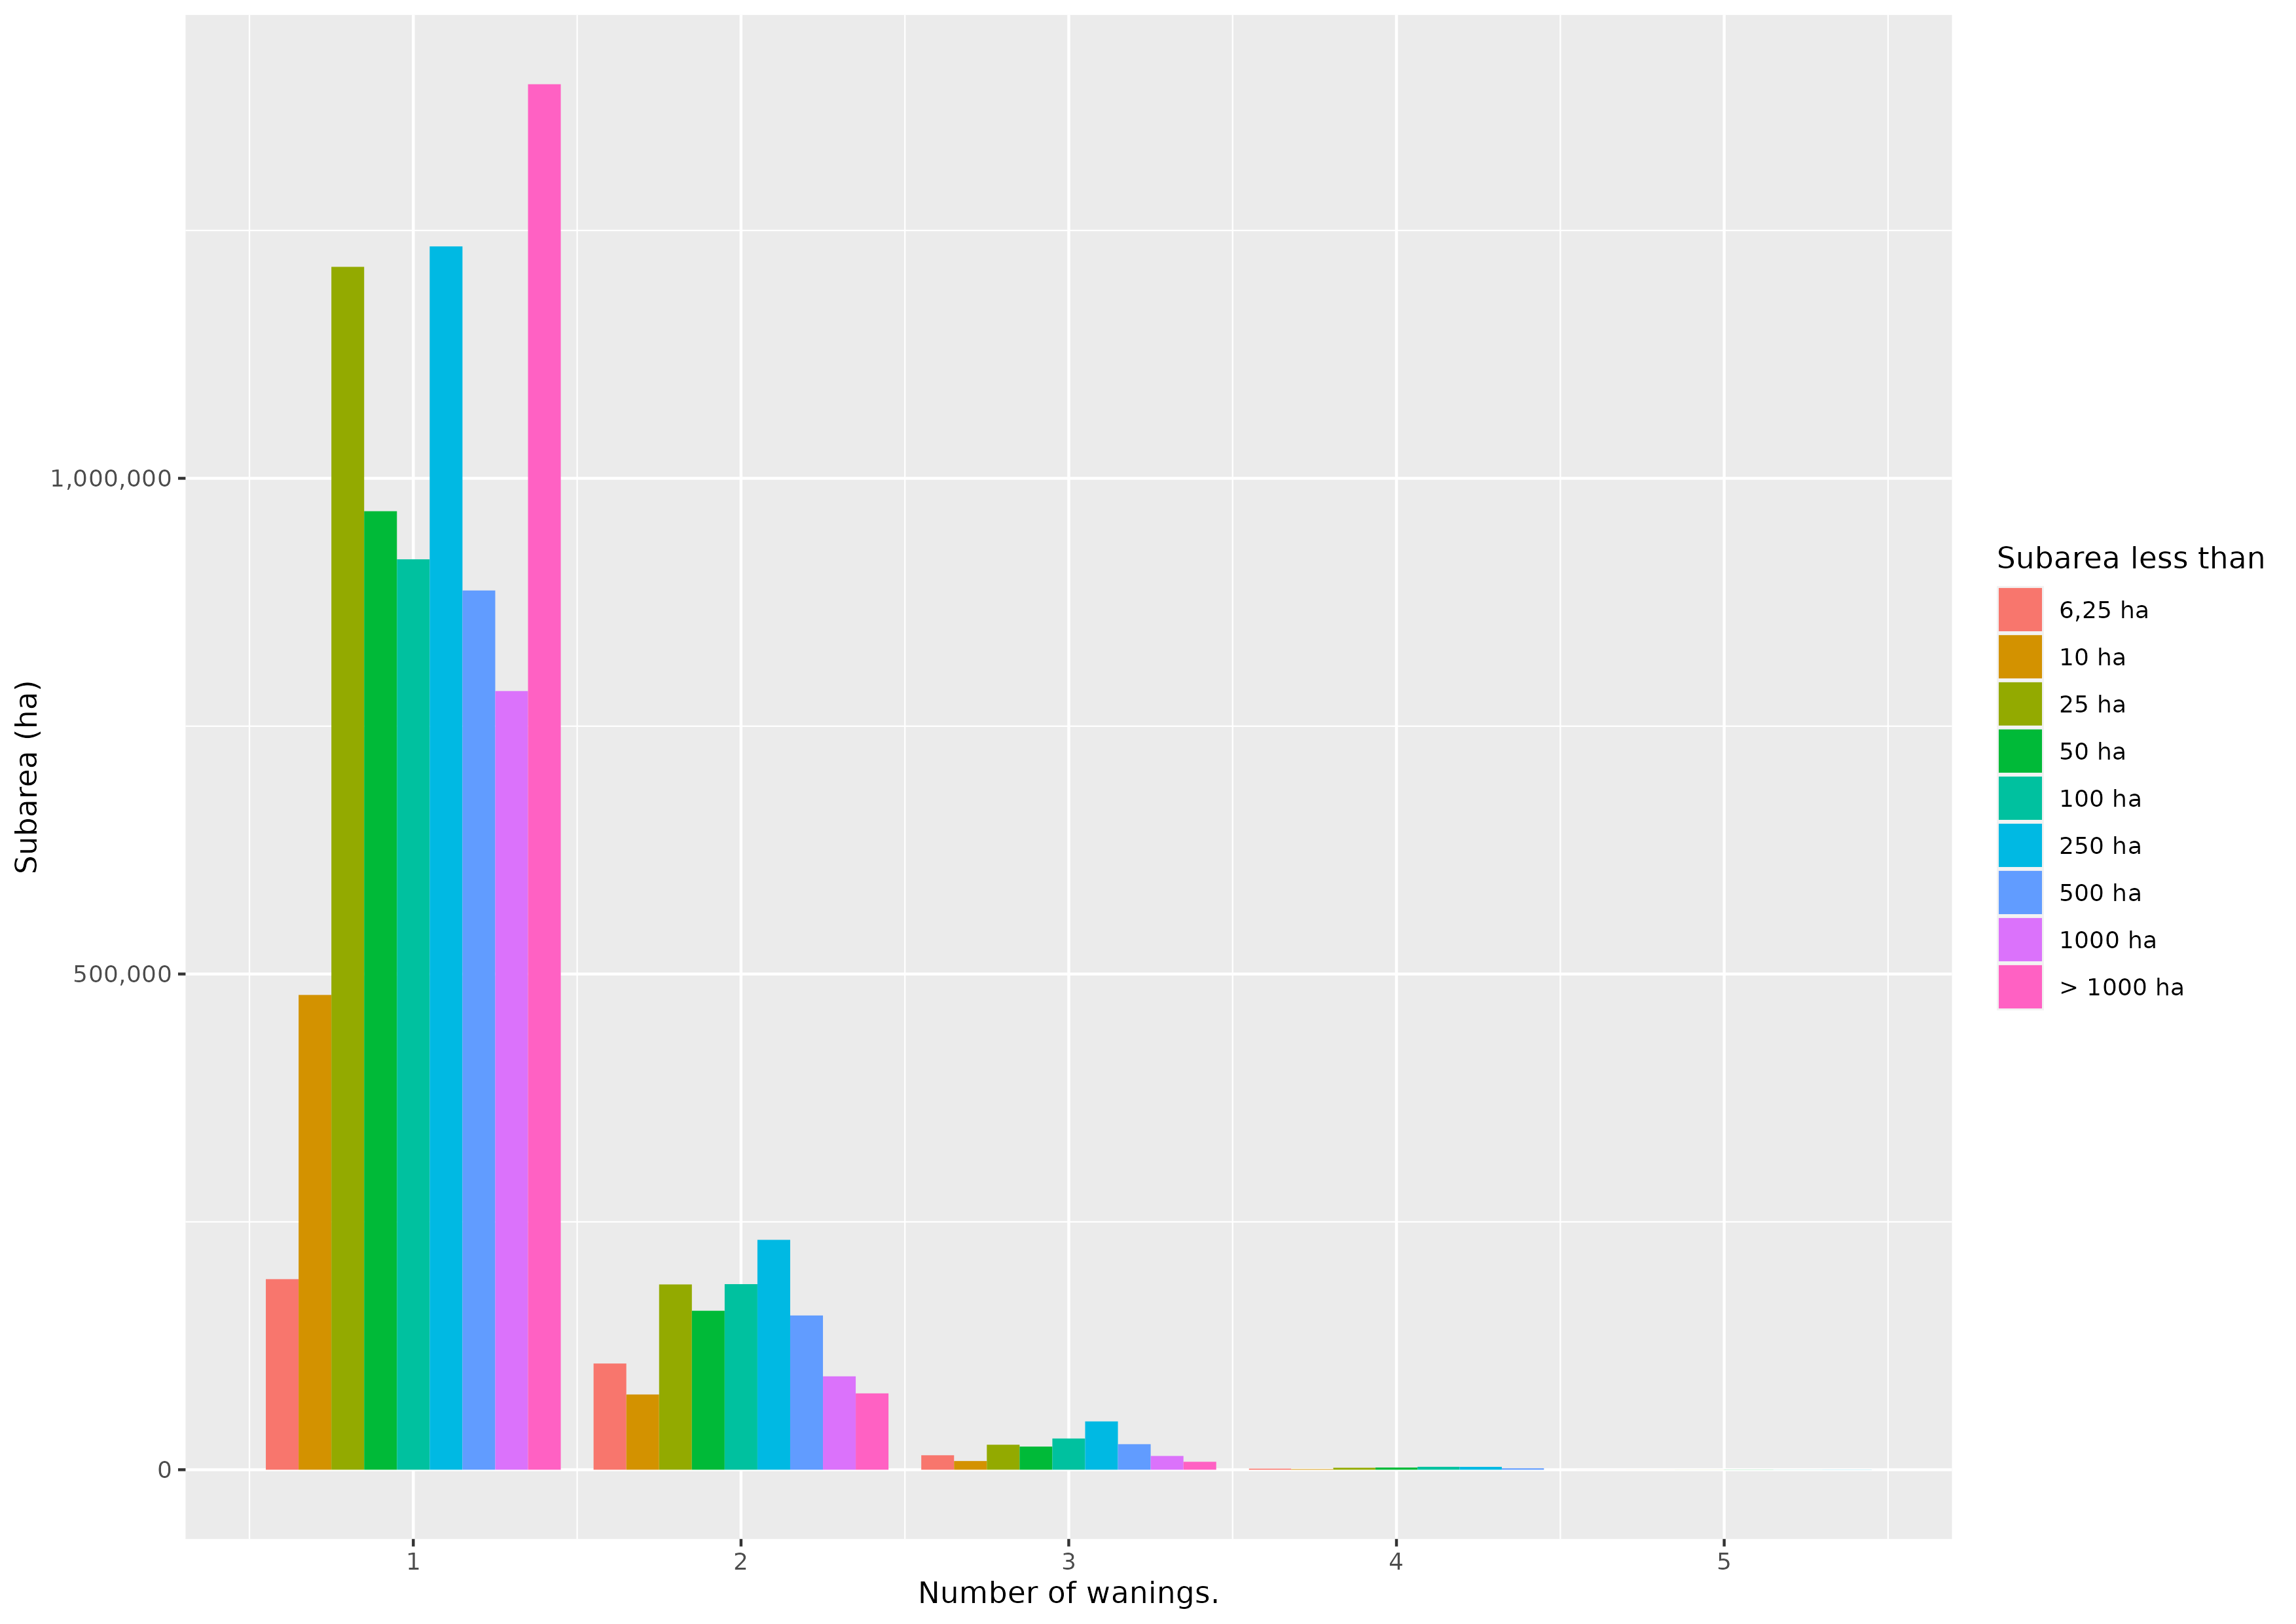
\includegraphics[width=1.0\textwidth]{./img_results/plot_deter_subarea_by_nwarnings.png}
\end{frame}

\begin{frame}
    \frametitle{DETER warnings by subarea}
    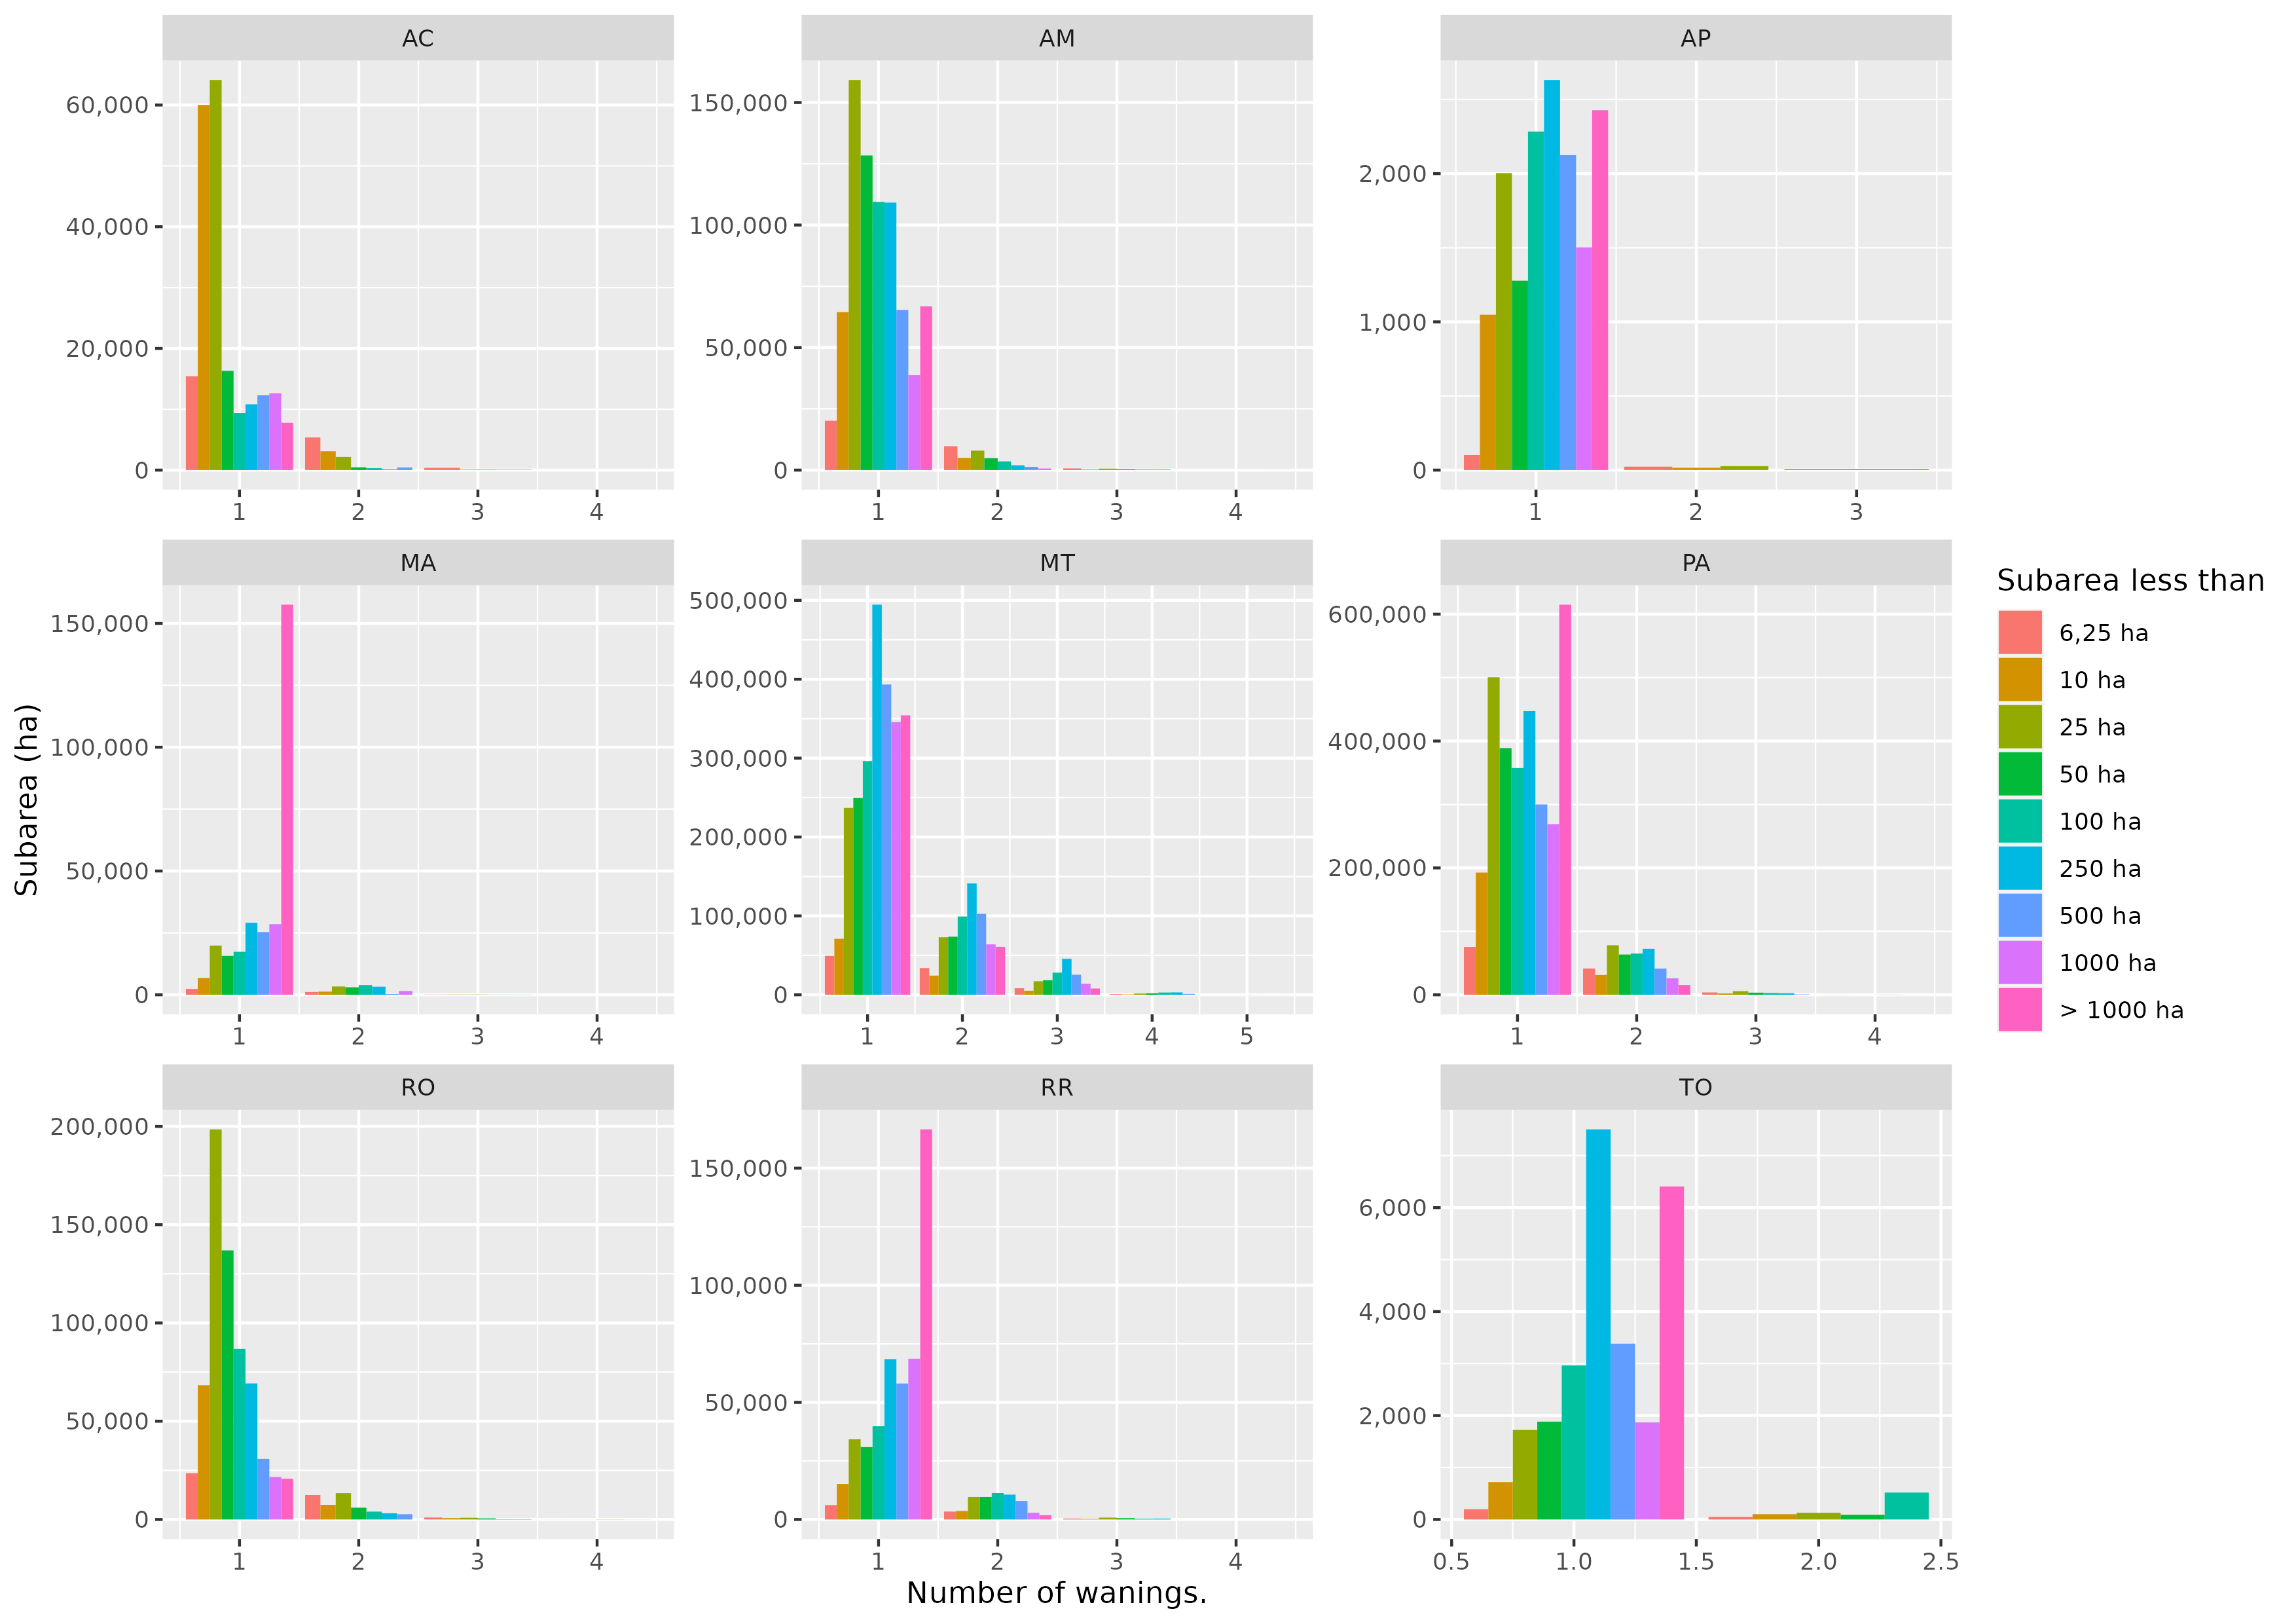
\includegraphics[width=1.0\textwidth]{./img_results/plot_deter_subarea_by_warnings_state.png}
\end{frame}

%%%%

\begin{frame}
    \frametitle{DETER subareas by size and days between warnings}
    \begin{itemize}
        \item The type is the first among the first and last DETER warnings.
        \item The color represents the year of the first warning.
    \end{itemize}
\end{frame}

\begin{frame}
    \frametitle{DETER subareas by size and days between warnings}
    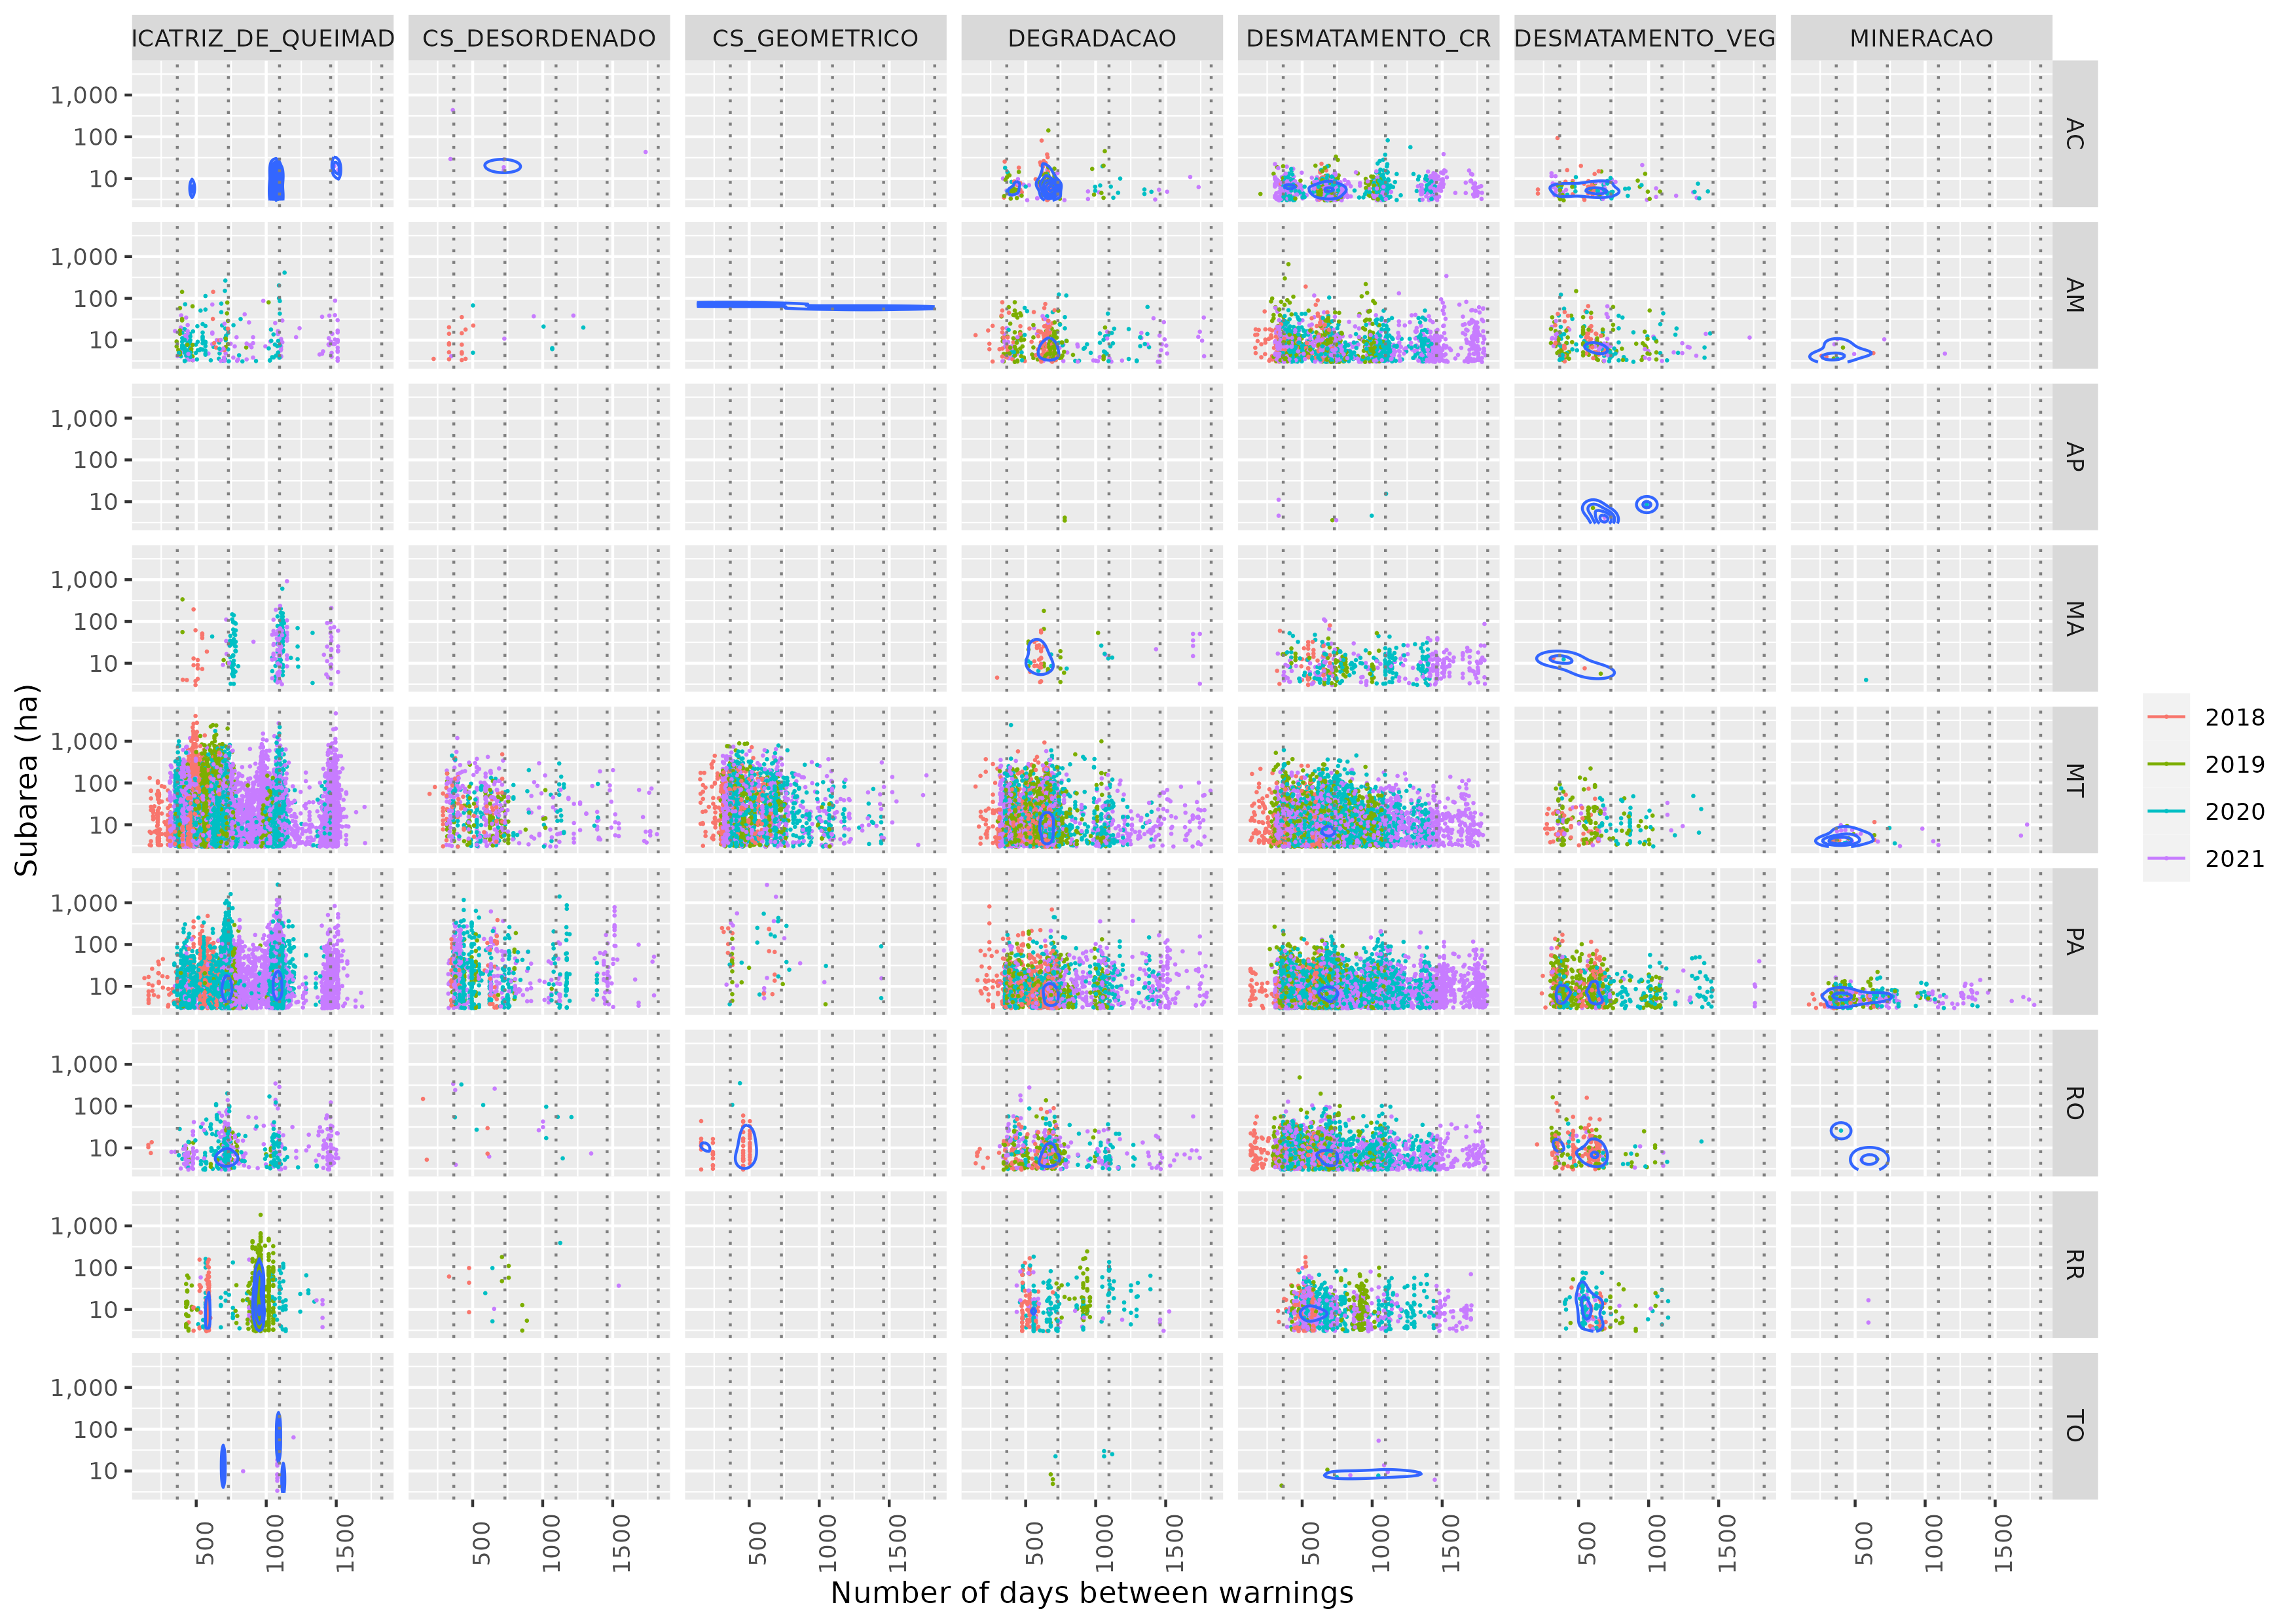
\includegraphics[width=1.0\textwidth]{./img_results/plot_deter_subarea_density_by_state_first-type_nwarnings.png}
\end{frame}

%%%%

\begin{frame}
    \frametitle{Time delay from first to last DETER warning}
    \begin{itemize}
        \item The following figure shows the distribution of time intervals
            between the first and last DETER warnings.
    \end{itemize}
\end{frame}

\begin{frame}
    \frametitle{Time delay from first to last DETER warning}
    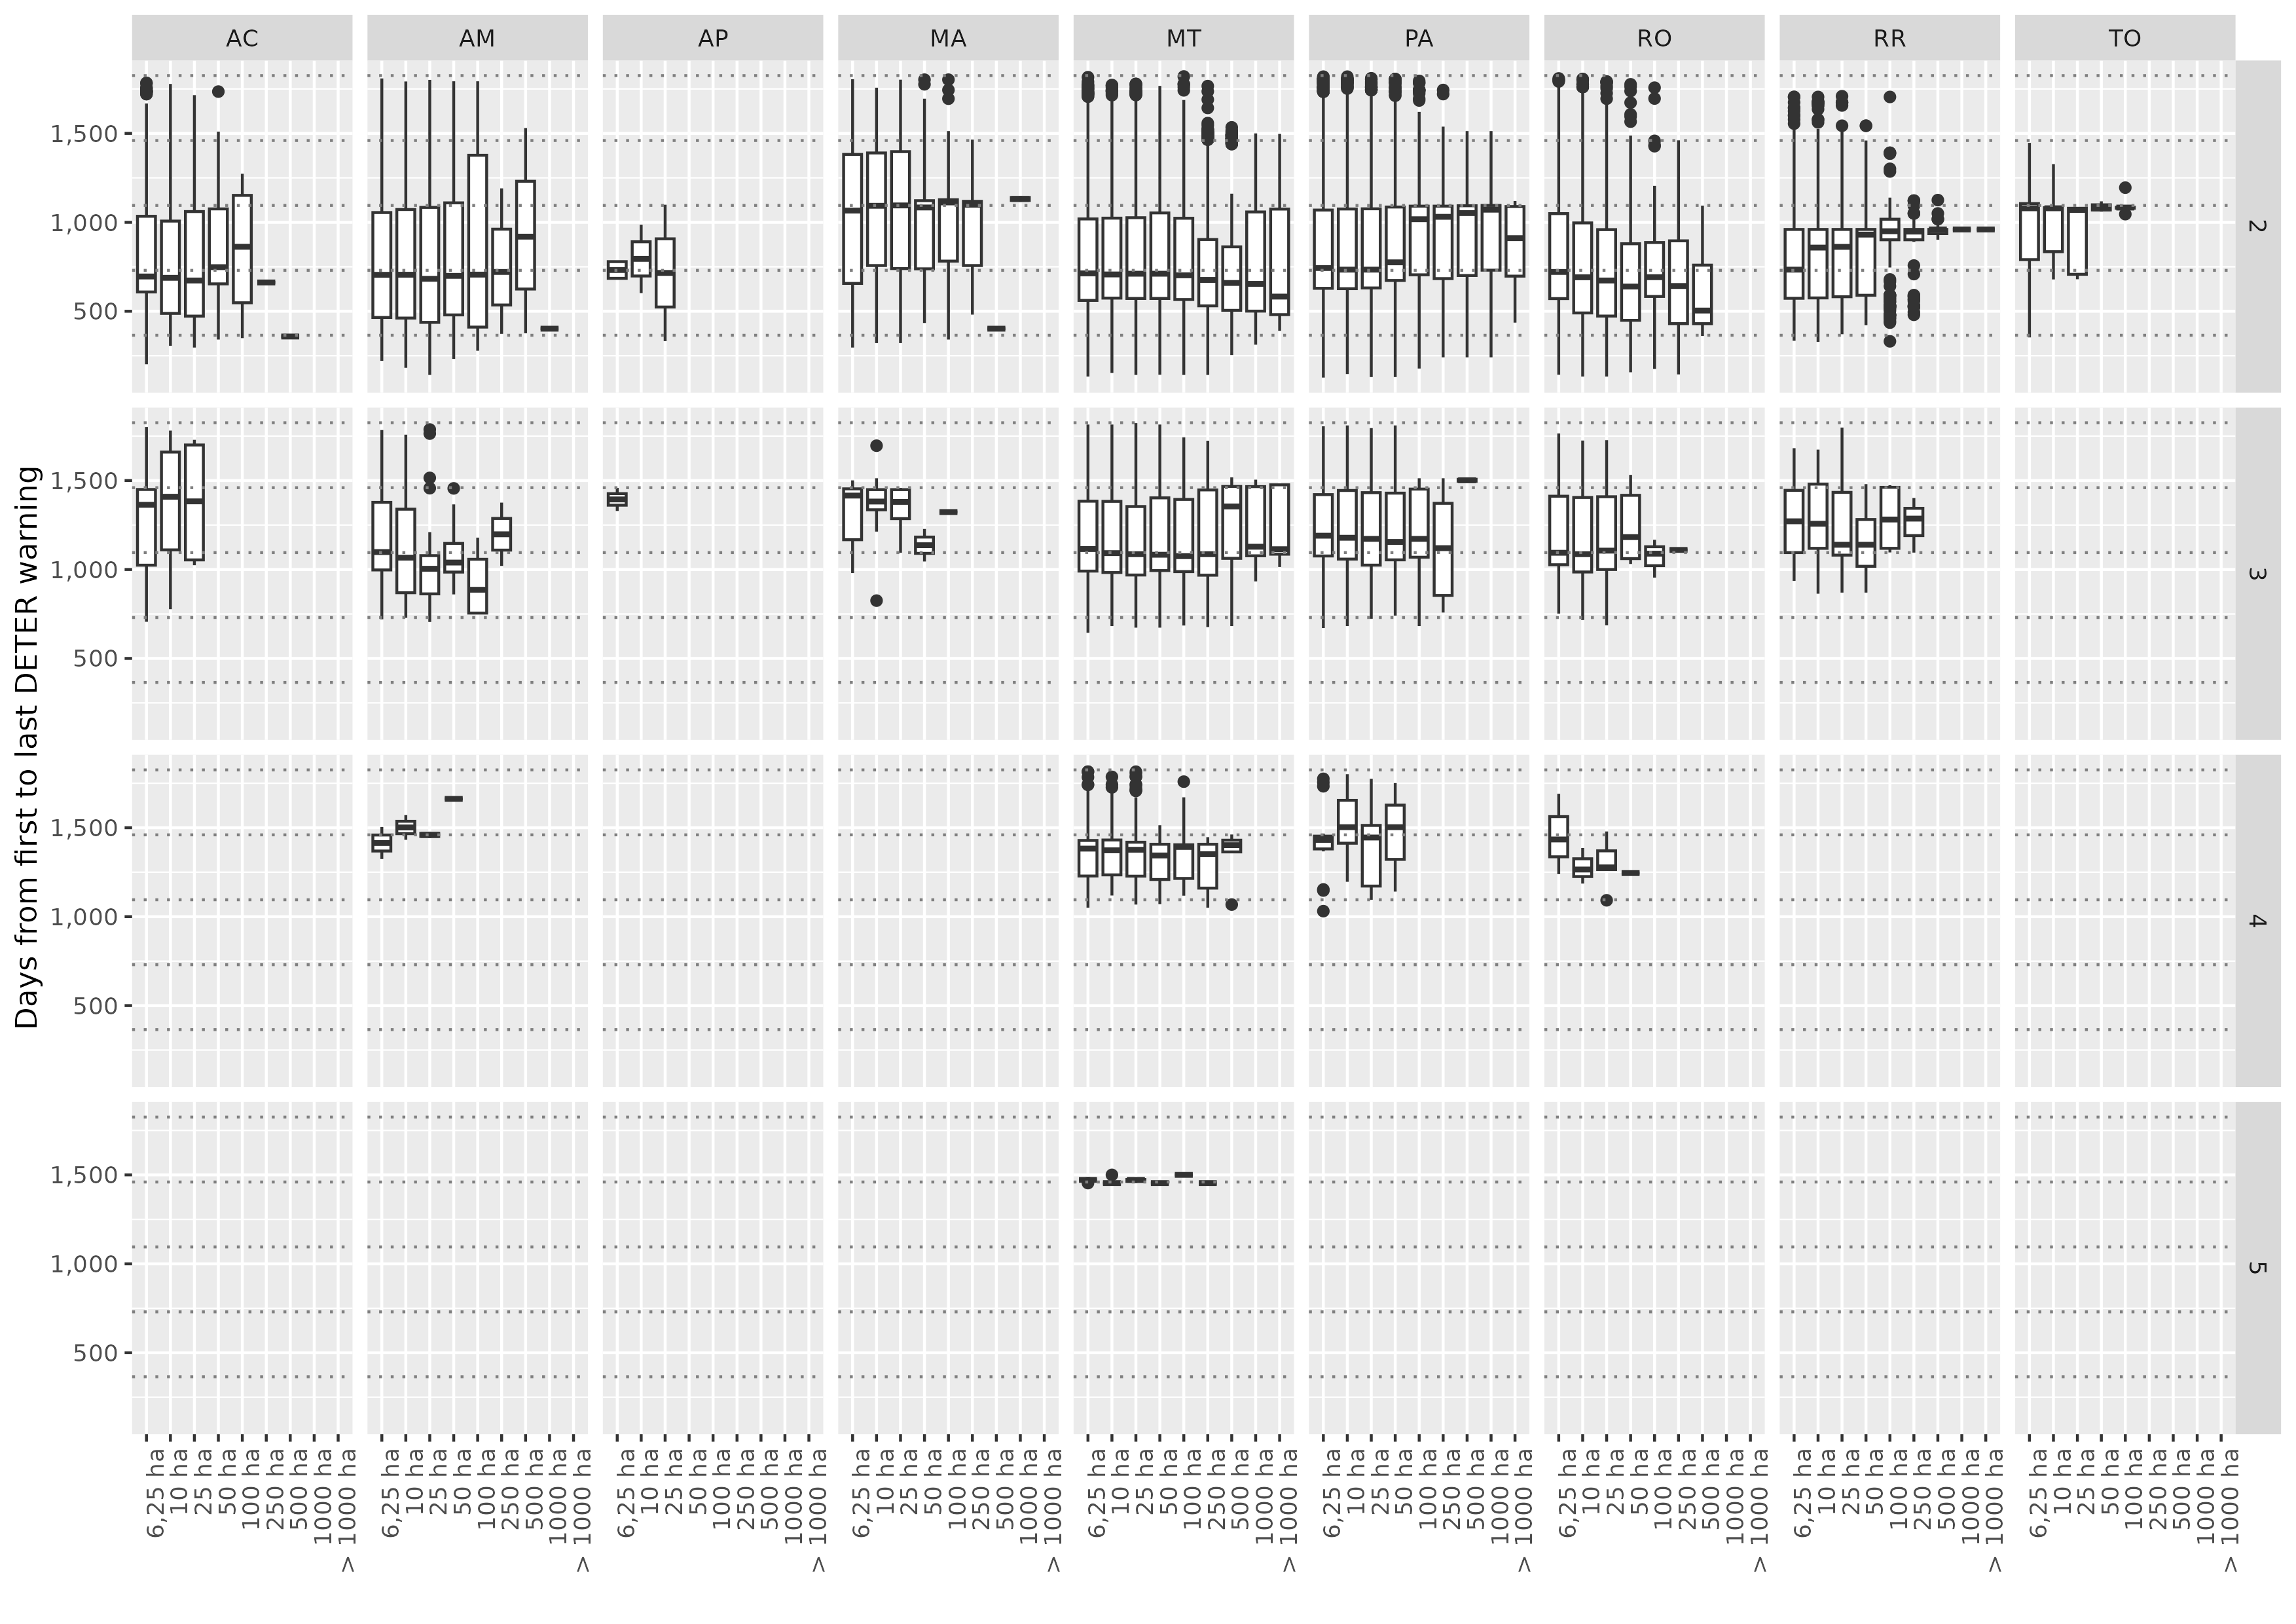
\includegraphics[width=1.0\textwidth]{./img_results/plot_deter_days_first_to_last.png}
\end{frame}

%%%%

\begin{frame}
    \frametitle{Trajectory of DETER's warnings}
    \begin{itemize}
        \item The following figures show the types of DETER subareas with more
            than one warning. 
        \item The trajectories also include the PRODES class (if any) 
            corresponding to each DETER subarea. The PRODES classes have the 
            suffix P. DETER's types don't have a suffix.
        \item The trajectories are chronologically ordered. The PRODES date
            is approximated to August 1st of the corresponding PRODES year 
            (PRODES' VIEWDATE isn't always the first date a class was 
            observed).
        \item These figures only show the order of the transitions and not the
            time between them.
    \end{itemize}
\end{frame}

\begin{frame}
    \frametitle{DETER warnings' trajectory (2 warnings) }
    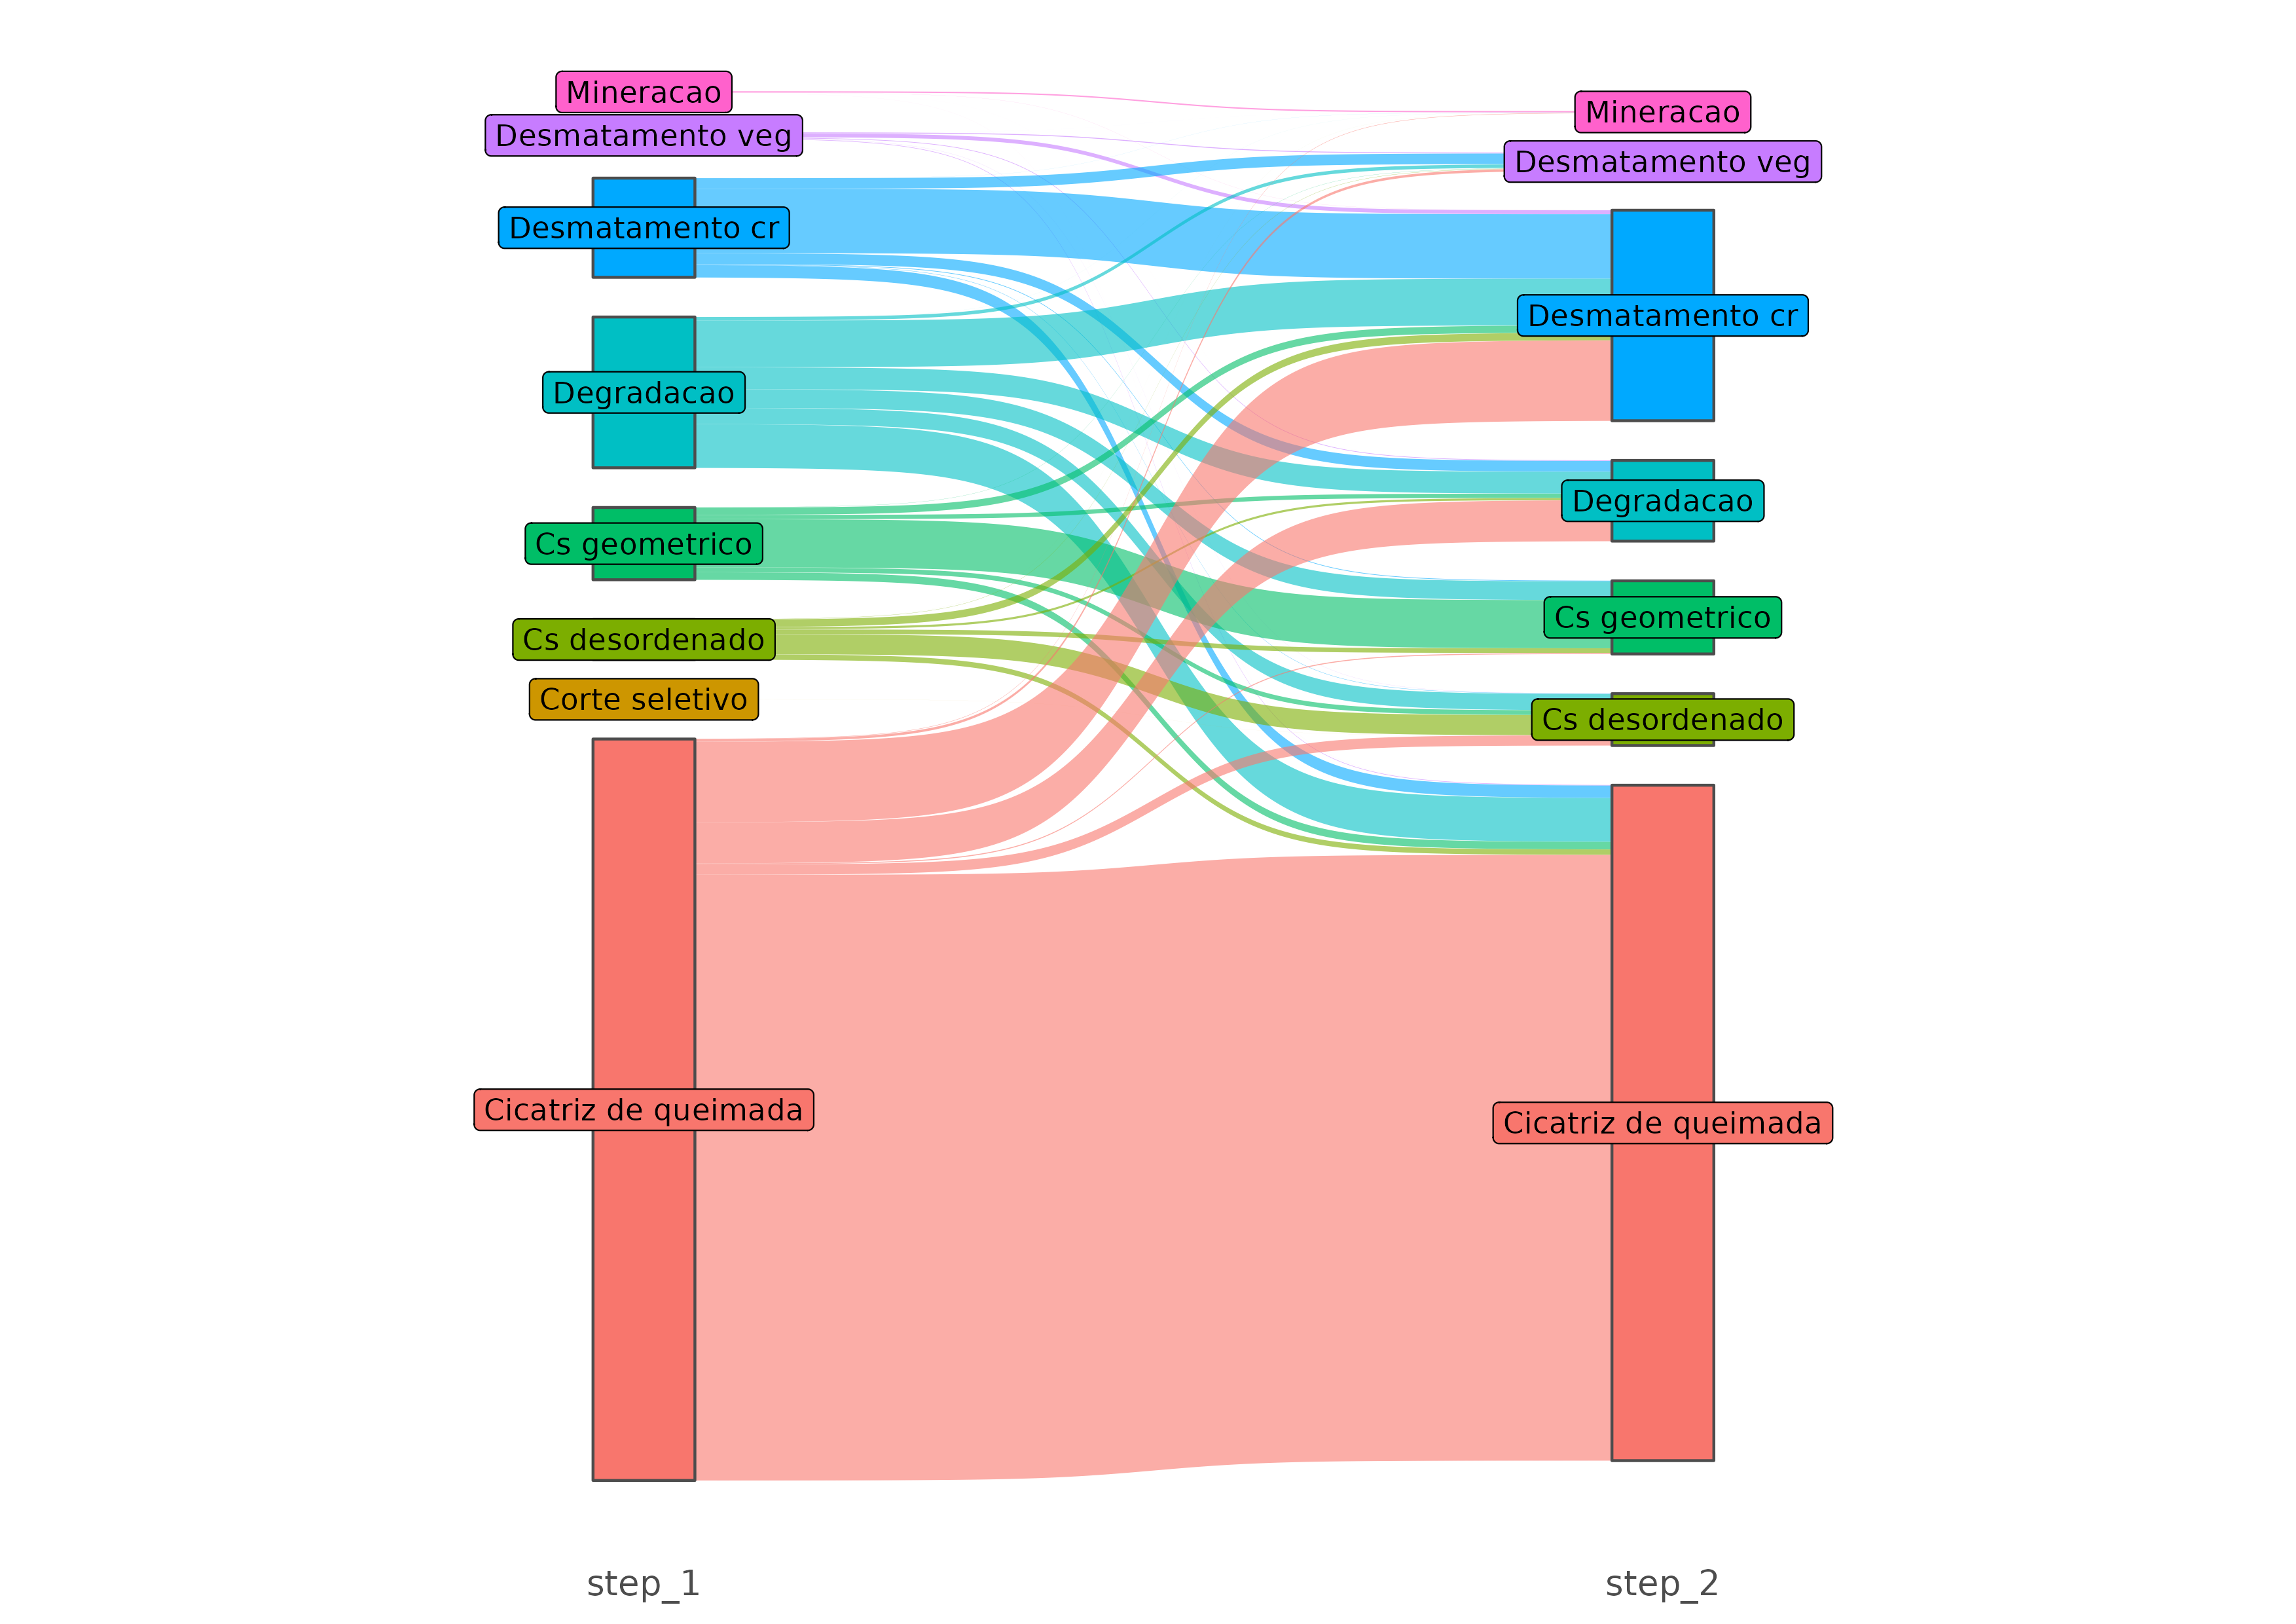
\includegraphics[width=1.0\textwidth]{./img_results/plot_deter_subarea_trajectory_2.png}
\end{frame}

\begin{frame}
    \frametitle{DETER warnings' trajectory (3 warnings) }
    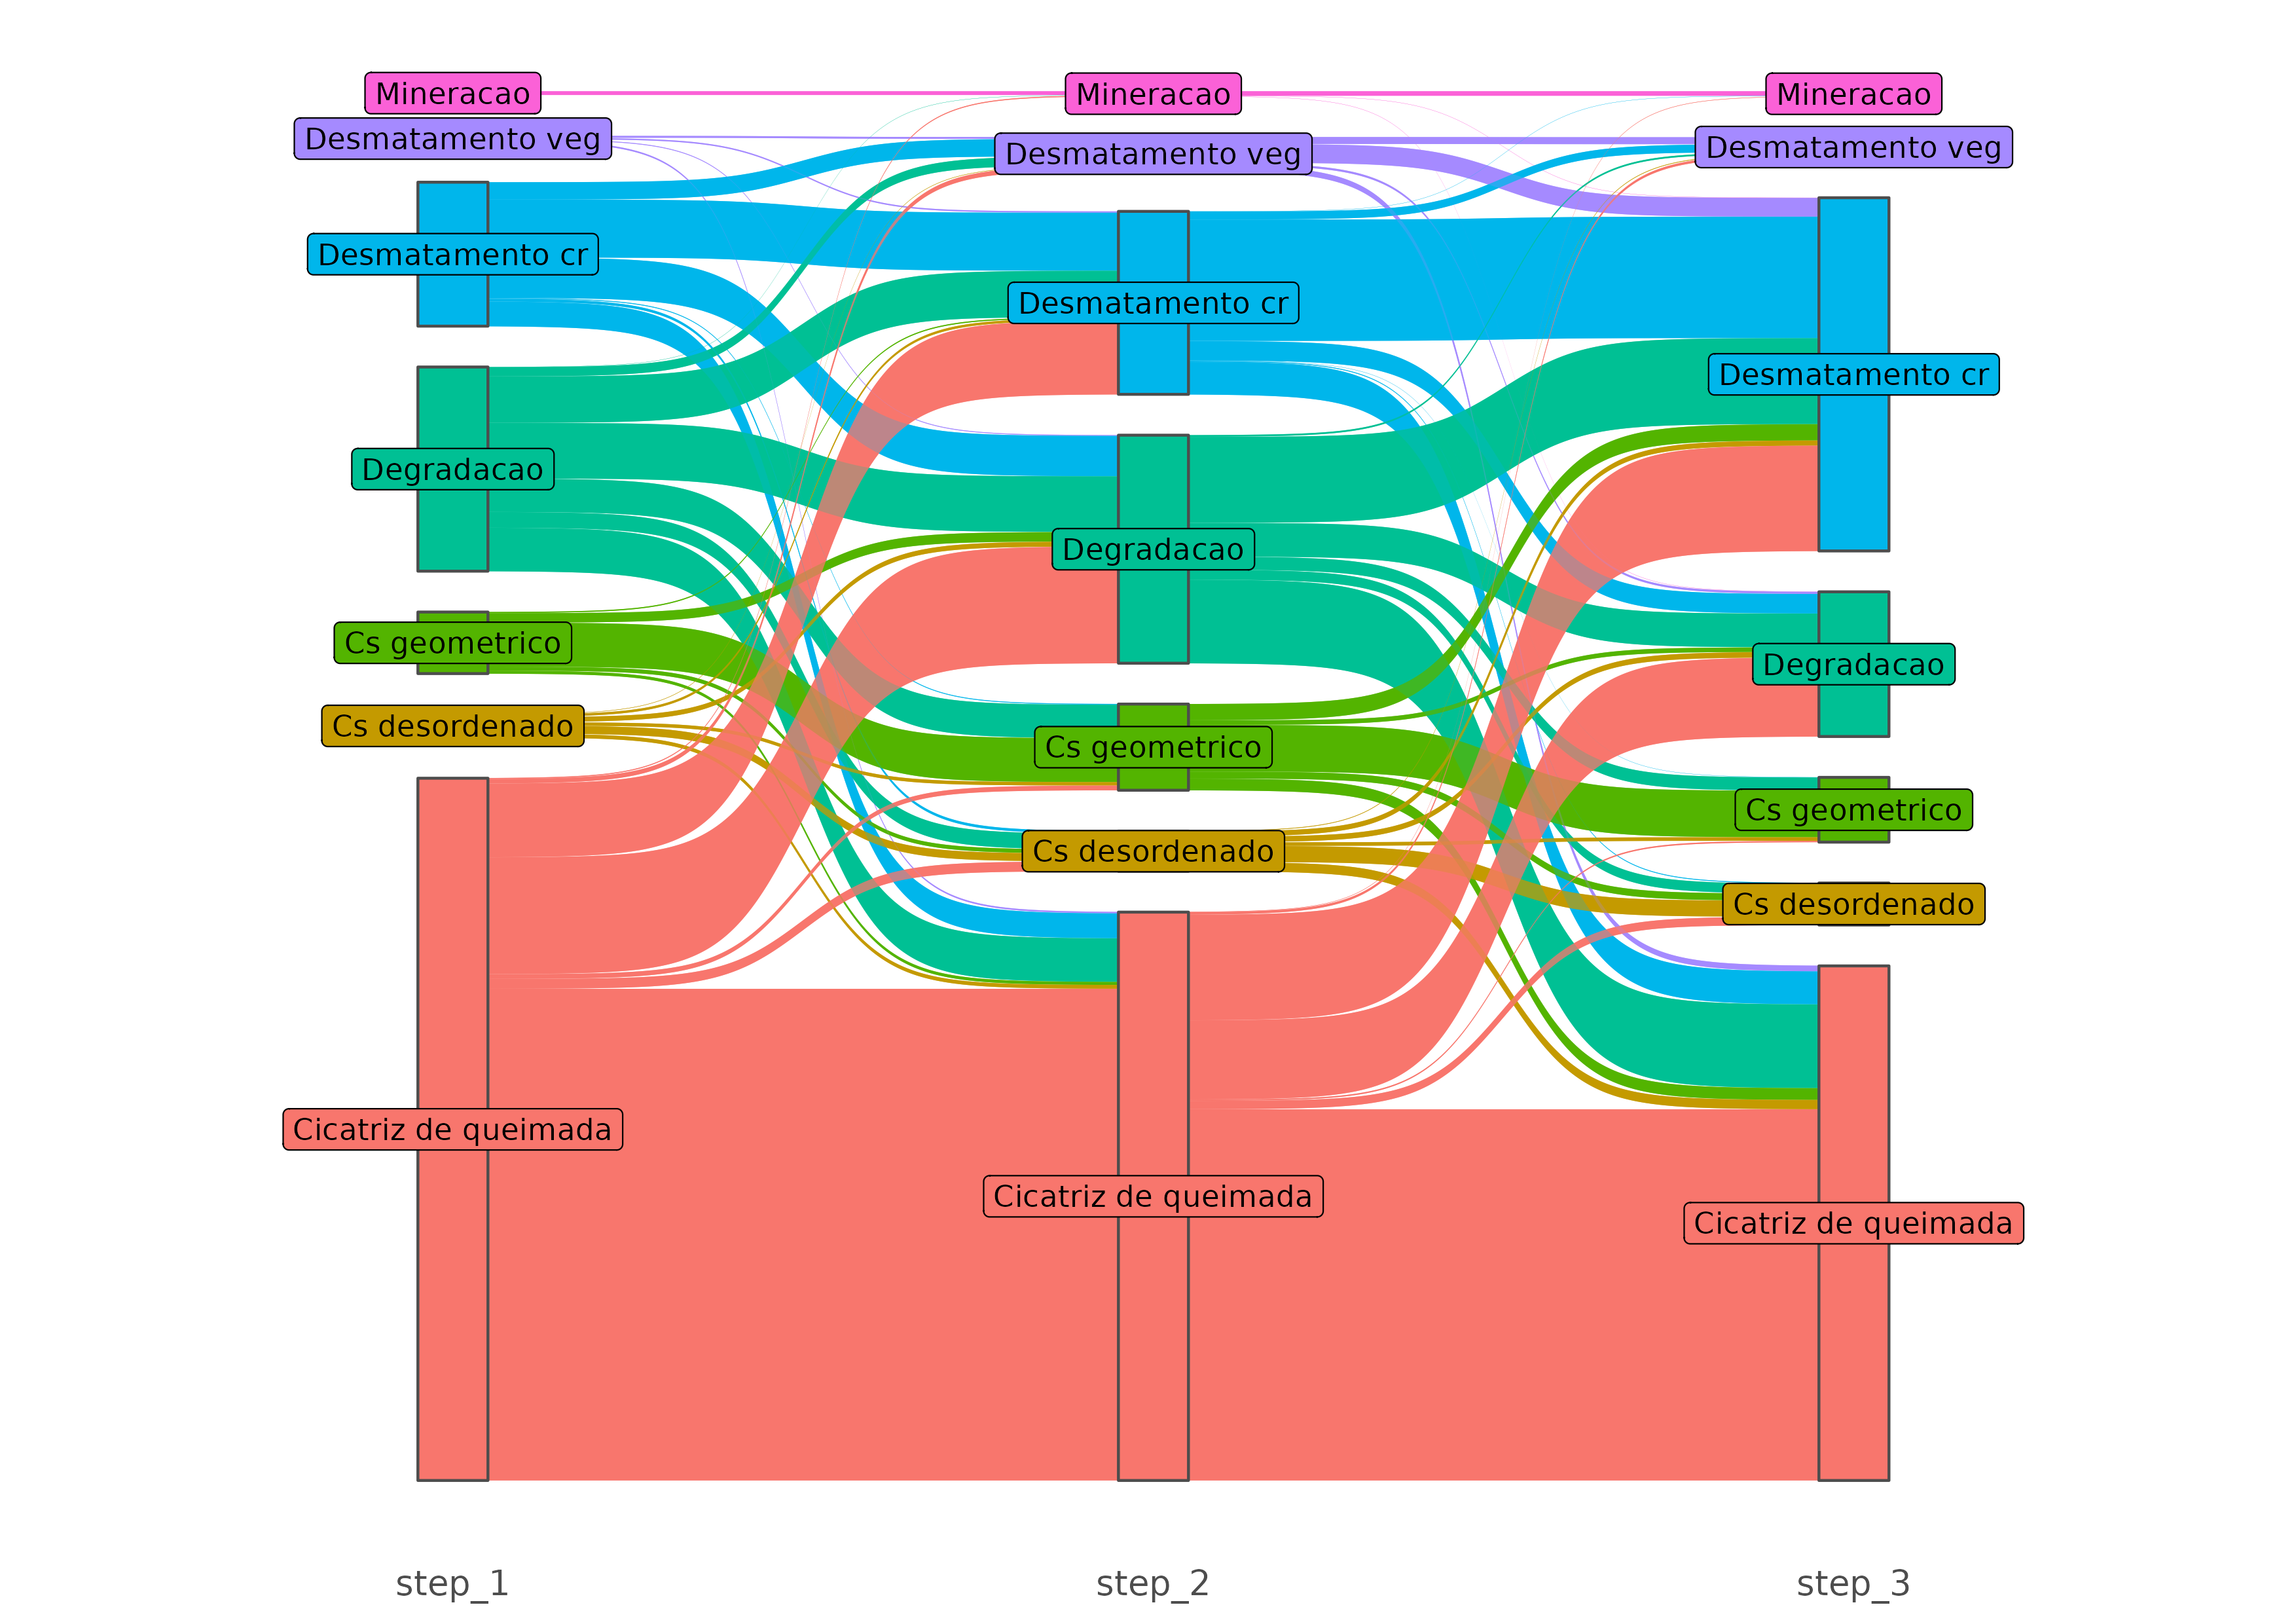
\includegraphics[width=1.0\textwidth]{./img_results/plot_deter_subarea_trajectory_3.png}
\end{frame}

\begin{frame}
    \frametitle{DETER warnings' trajectory (4 warnings) }
    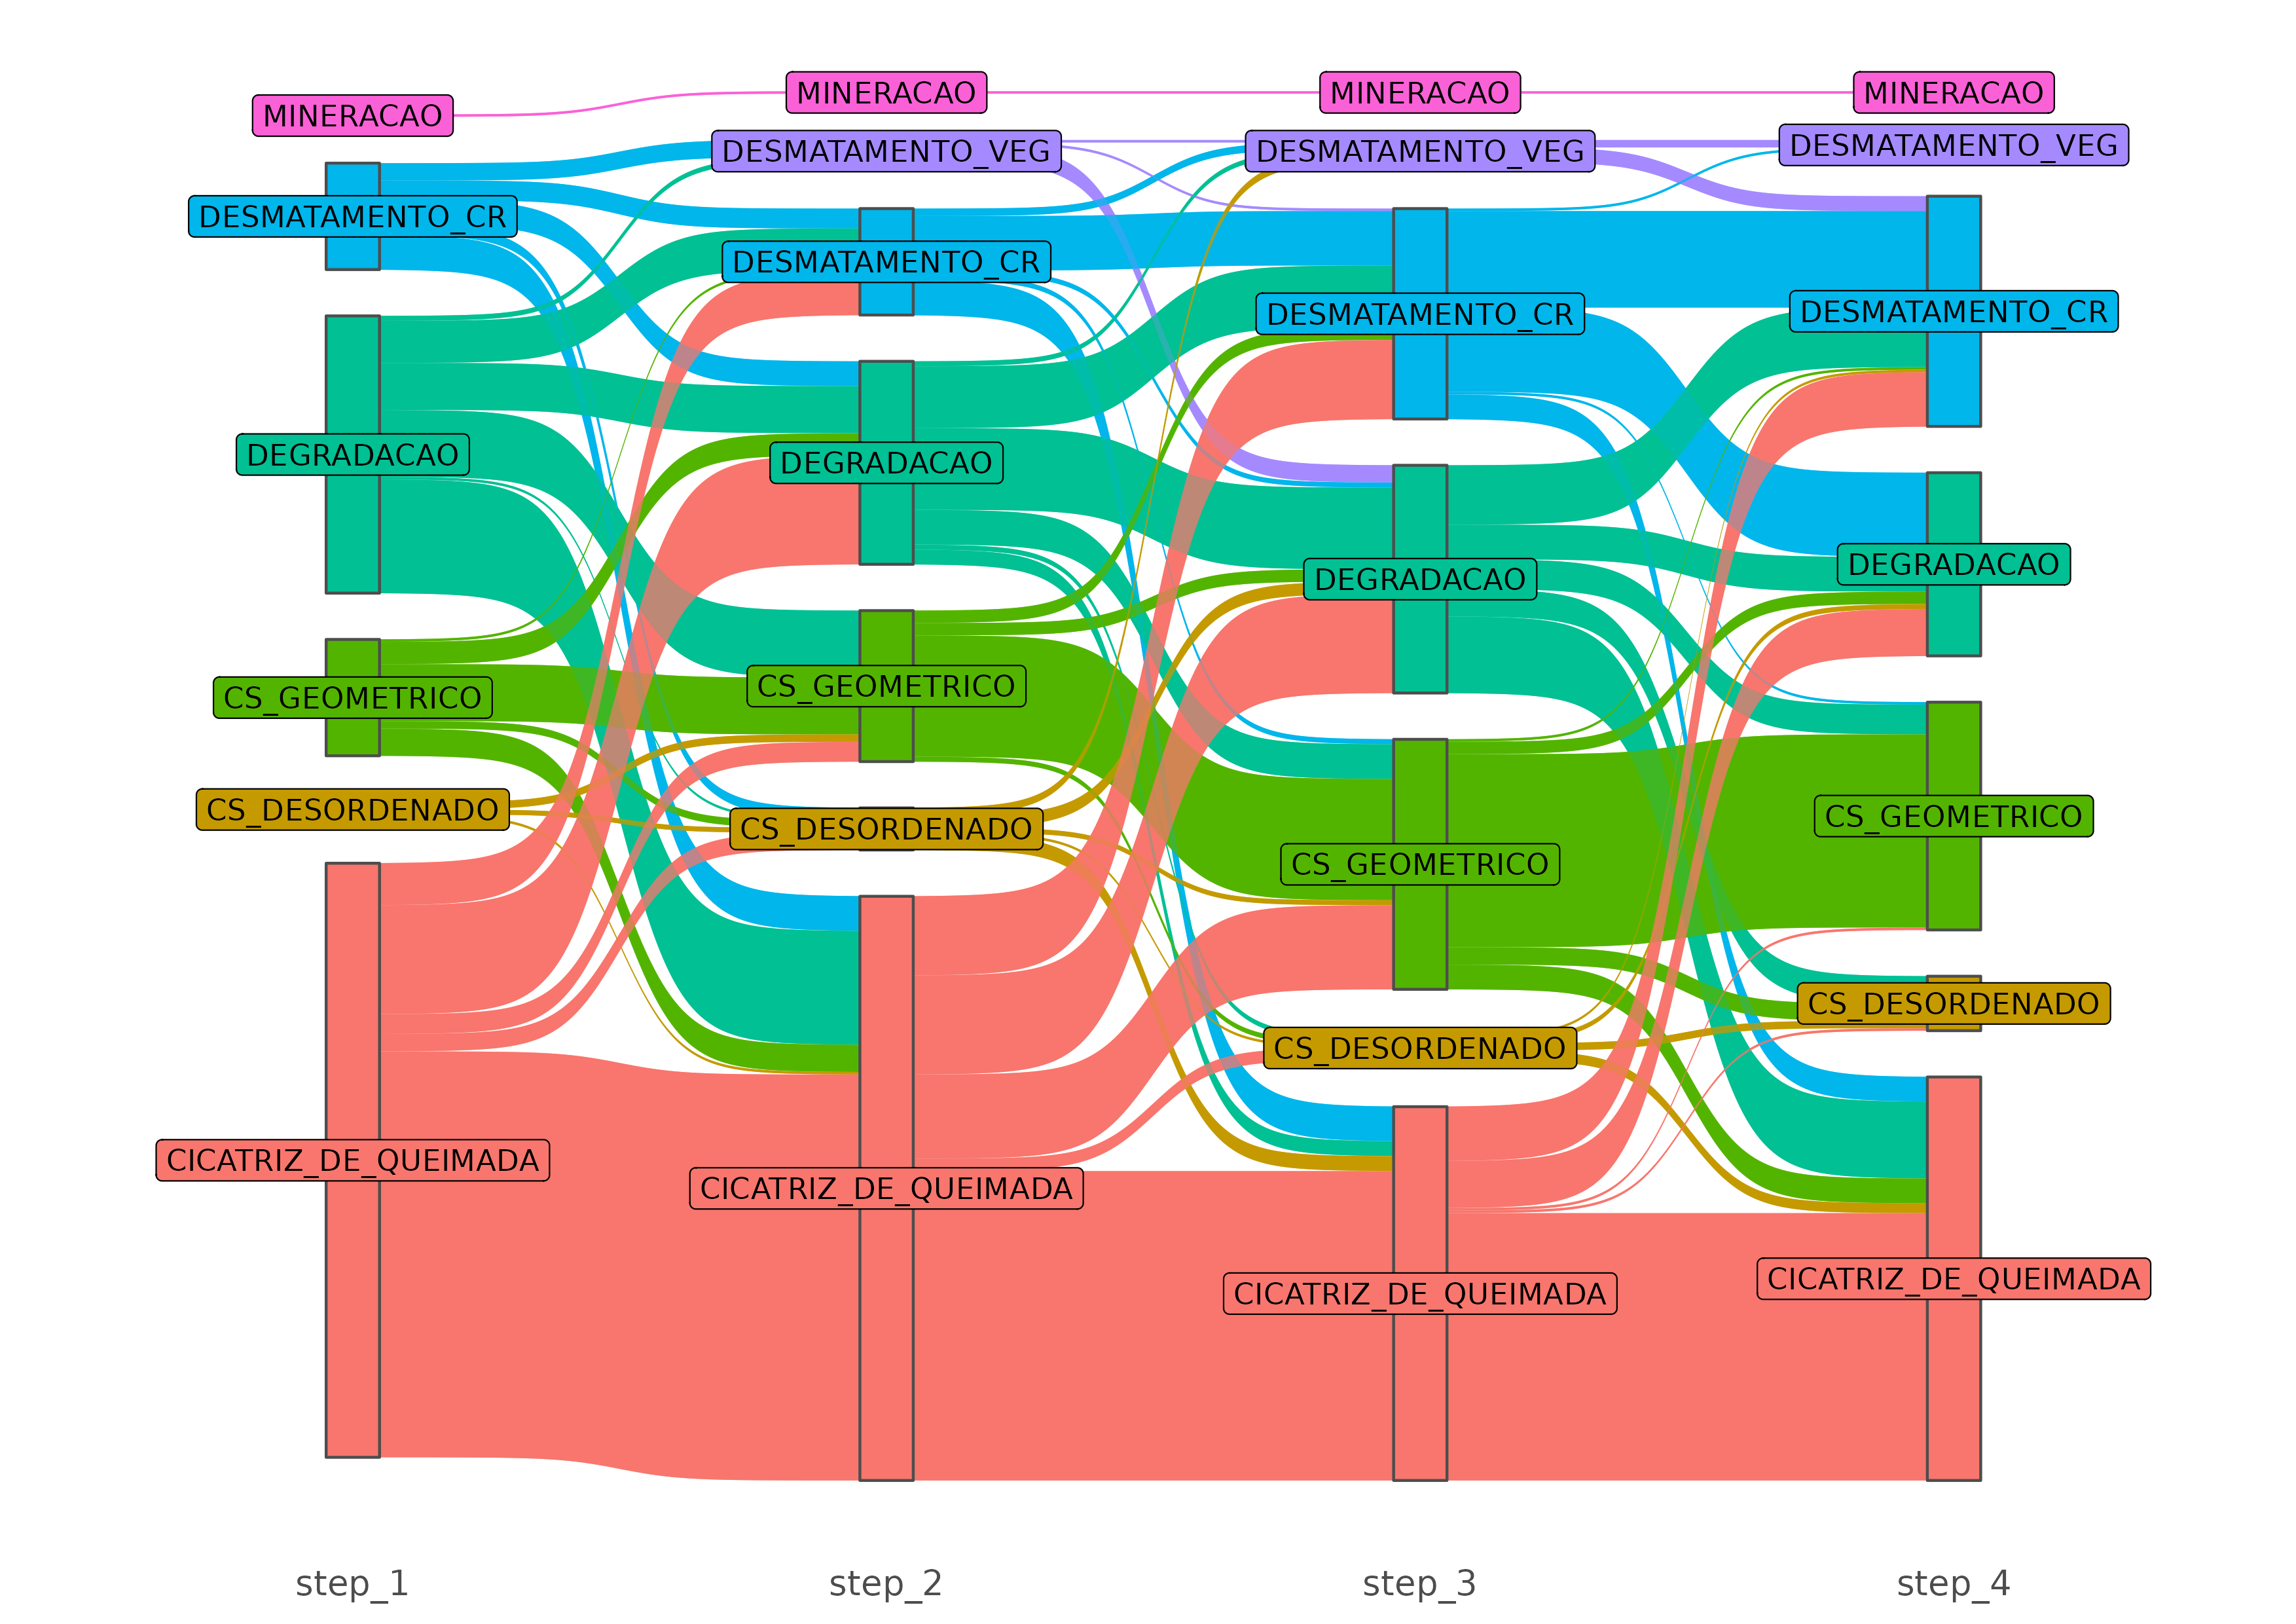
\includegraphics[width=1.0\textwidth]{./img_results/plot_deter_subarea_trajectory_4.png}
\end{frame}

\begin{frame}
    \frametitle{DETER warnings' trajectory (5 warnings) }
    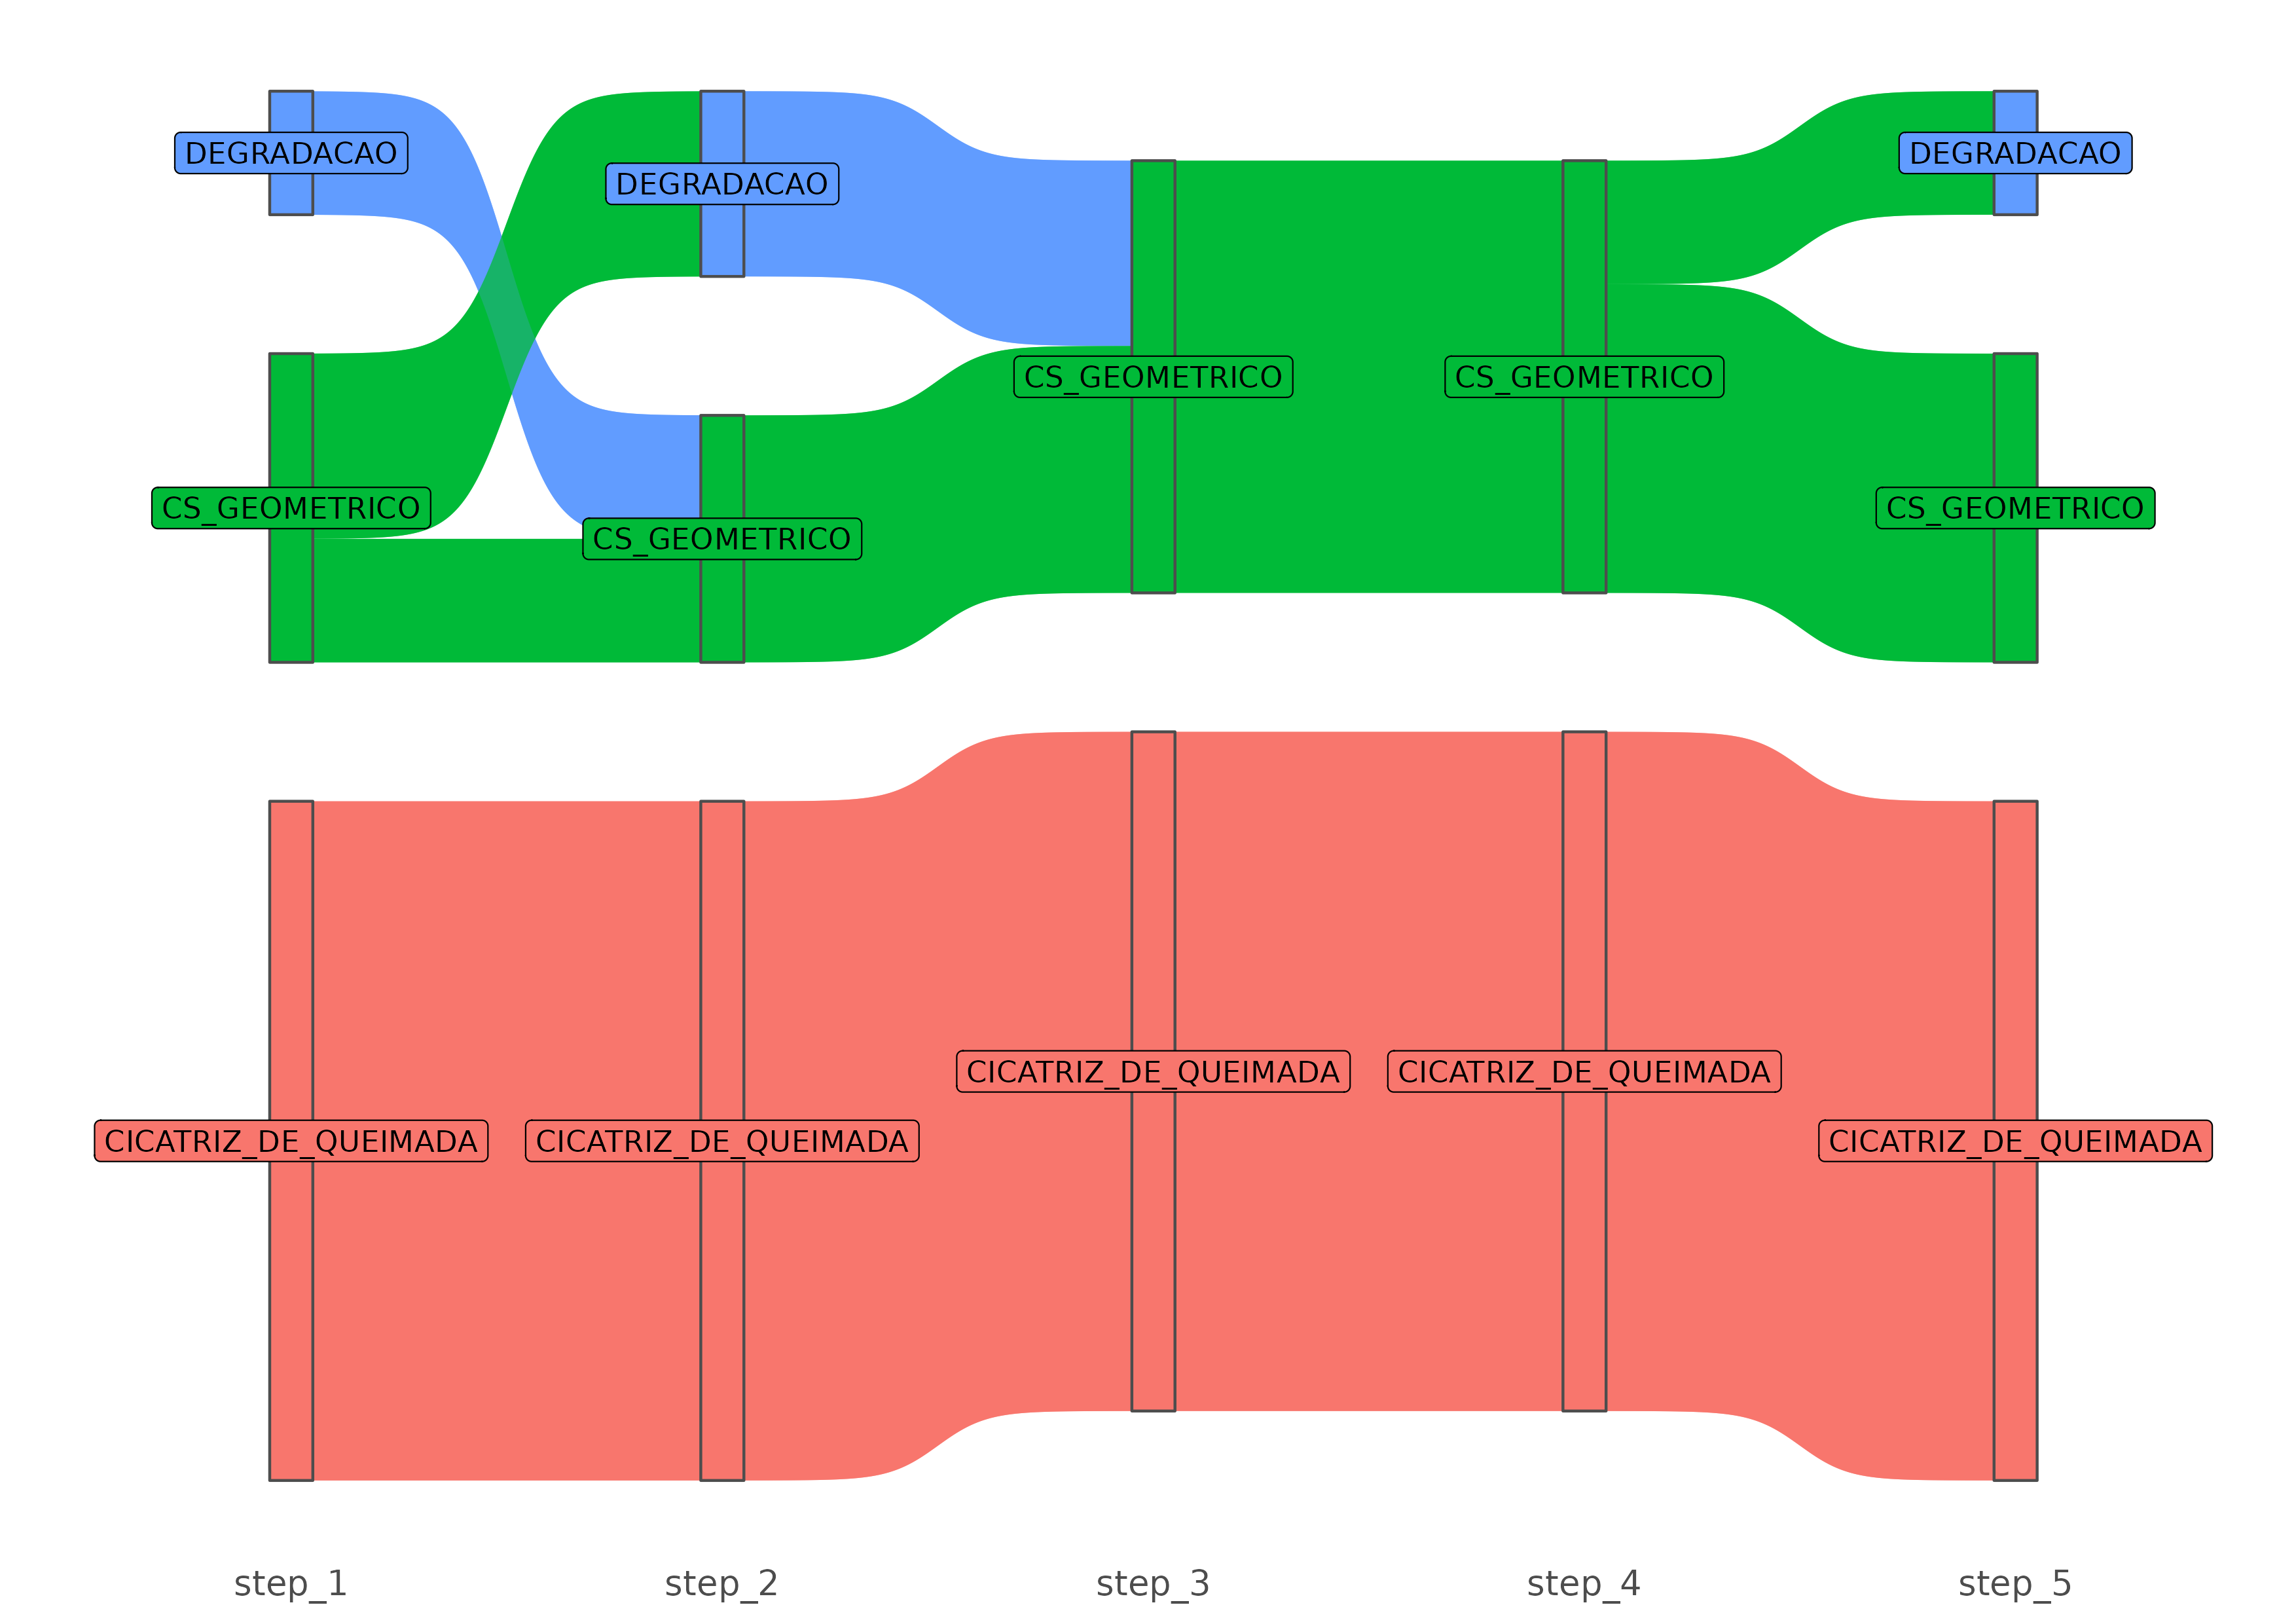
\includegraphics[width=1.0\textwidth]{./img_results/plot_deter_subarea_trajectory_5.png}
\end{frame}

\begin{frame}
    \frametitle{DETER warnings' trajectory (6 warnings) }
    \includegraphics[width=1.0\textwidth]{./img_results/plot_deter_subarea_trajectory_6.png}
\end{frame}


%%%%%%%%%%%%%%%%%%%%%%%%%%%%%%%%%%%%%%%%%%%%%%%%%%%%%%%%%%%%%%%%%%%%%%%%%%%%%%%
% End.
%%%%%%%%%%%%%%%%%%%%%%%%%%%%%%%%%%%%%%%%%%%%%%%%%%%%%%%%%%%%%%%%%%%%%%%%%%%%%%%

\begin{frame}
    Questions?
\end{frame}



%%%%%%%%%%%%%%%%%%%%%%%%%%%%%%%%%%%%%%%%%%%%%%%%%%%%%%%%%%%%%%%%%%%%%%%%%%%%%%%
% Other
%%%%%%%%%%%%%%%%%%%%%%%%%%%%%%%%%%%%%%%%%%%%%%%%%%%%%%%%%%%%%%%%%%%%%%%%%%%%%%%

%%%%%%%%%%%%%%%%%%%%%%%%%%%%%%%%%%%%%%%%%%%%%%%%%%%%%%%%%%%%%%%%%%%%%%%%%%%%%%%
\section{References}
%%%%%%%%%%%%%%%%%%%%%%%%%%%%%%%%%%%%%%%%%%%%%%%%%%%%%%%%%%%%%%%%%%%%%%%%%%%%%%%

\begin{frame}[t, allowframebreaks]
    \frametitle{References}
    \bibliographystyle{abbrv}
    \bibliography{project}
\end{frame}

\end{document}

